\documentclass[11pt, a4paper]{report}
\usepackage[english]{babel}
\usepackage[T1]{fontenc}
\usepackage[utf8]{inputenc}
\usepackage{pdfpages}

\DeclareUnicodeCharacter{2010}{-}% support older LaTeX versions
\usepackage{wallpaper}
\usepackage{palatino}
\usepackage{changepage}
\usepackage{mhchem} % for isotope nomeclature support
% Setup captions
%\captionstyle[\centering]{\centering}
%\changecaptionwidth
%\captionwidth{0.8\linewidth}

% Protect against widows and orphans
%\clubpenalty=10000
%\widowpenalty=10000

%\linespread{1.2}

%\raggedbottom

%\chapterstyle{ger}

%\maxsecnumdepth{subsection}

%%  Setup fancy style quotation
%%  ==================================================================
%\usepackage{tikz}
%\usepackage{framed}

%\newcommand*\quotefont{\fontfamily{fxl}} % selects Libertine for quote font

% Make commands for the quotes
%\newcommand*{\openquote}{\tikz[remember picture,overlay,xshift=-15pt,yshift=-10pt]
%     \node (OQ) {\quotefont\fontsize{60}{60}\selectfont``};\kern0pt}
%\newcommand*{\closequote}{\tikz[remember picture,overlay,xshift=15pt,yshift=5pt]
%     \node (CQ) {\quotefont\fontsize{60}{60}\selectfont''};}

% select a colour for the shading
%\definecolor{shadecolor}{rgb}{1,1,1}

% wrap everything in its own environment
%\newenvironment{shadequote}% 
%{\begin{snugshade}\begin{quote}\openquote}
%{\hfill\closequote\end{quote}\end{snugshade}}



%% MY STUFF


%% Language and font encodings

%% Sets page size and margins
%\usepackage[a4paper,top=2.5cm,bottom=2cm,left=2.5cm,right=2.5cm,marginparwidth=1.75cm]{geometry}
\usepackage{graphicx}
\usepackage{caption}
\usepackage{subcaption}
\captionsetup{font={small},skip=0.25\baselineskip}
\captionsetup[subfigure]{font={bf, footnotesize}, skip=1pt, singlelinecheck=false}
\graphicspath{{./plots/}{./figures/}}

%\fancypagestyle{title}{%
%  \setlength{\headheight}{120pt}%
%  \fancyhf{}% No header/footer
%  \renewcommand{\headrulewidth}{0pt}% No header rule
%  \renewcommand{\footrulewidth}{0pt}% No footer rule
%  %\fancyhead[L]{\small\begin{tabular}{@{}l}\includegraphics[width=0.15\textwidth]{ku}\end{tabular}}
%   % \fancyhead[C]{\small\begin{tabular}{@{}l}\includegraphics[width=0.6\textwidth]{PROSCION}\end{tabular}}
%  %\fancyhead[R]{\small\begin{tabular}{@{}r}\includegraphics[width=0.15\textwidth]{naturvidenskab}\end{tabular}}
%}%


%\usepackage{amsmath}
%\usepackage[format=plain]{caption}
\usepackage{subcaption}
\usepackage{float} % force float
\usepackage[nottoc]{tocbibind}
%\usepackage[margin=-50pt]{caption}
%\usepackage[colorinlistoftodos]{todonotes}
\usepackage[colorlinks=true, allcolors=blue]{hyperref}
\usepackage{cleveref} % for enumerate/itemize item referencing

%\setlength{\parindent}{4em}
%\setlength{\parskip}{1em}
%\usepackage{mathpazo} % Use the Palatino font
\usepackage{parskip}% http://ctan.org/pkg/parskip
\usepackage{xspace}
\usepackage{wrapfig}
\usepackage[export]{adjustbox}
\usepackage{textcomp}
\usepackage[bottom]{footmisc}


\usepackage{titling}
\newcommand{\subtitle}[1]{%
  \posttitle{%
    \par\end{center}
    \begin{center}\large#1\end{center}
    \vskip0.5em}%
}

\renewcommand\thesubfigure{\arabic{subfigure}}  
\captionsetup{format=hang,labelsep=space,indention=-2cm,labelfont=bf,width=.9\textwidth,skip=.5\baselineskip}
%\captionsetup[sub]{labelfont=bf, labelsep=period,labelformat=simple, subrefformat=brace}


\usepackage{listings}
\lstset{basicstyle=\ttfamily,
  showstringspaces=false,
  commentstyle=\color{red},
  keywordstyle=\color{blue}
}

\makeatletter
\renewcommand\p@subfigure{\thefigure\,}
\renewcommand\thesubfigure{\alph{subfigure})}
% If desired for table as well:
% \renewcommand\p@subtable{\thetable\,}
% \renewcommand\thesubtable{\alph{subtable})}
\DeclareCaptionLabelFormat{mysublabelfmt}{\alph{sub\@captype}}
\makeatother

\renewcommand{\baselinestretch}{1.5}
\DeclareCaptionSubType*[arabic]{figure}



%\makeatletter
%\renewcommand\thesection{}
%\renewcommand\thesubsection{\@arabic\c@subsection}
%\makeatother

\usepackage{mathtools}
\usepackage{sectsty}

\chapternumberfont{\LARGE} 
\chaptertitlefont{\LARGE}


\DeclarePairedDelimiter\abs{\lvert}{\rvert}%
\DeclarePairedDelimiter\norm{\lVert}{\rVert}%

% Swap the definition of \abs* and \norm*, so that \abs
% and \norm resizes the size of the brackets, and the 
% starred version does not.
\makeatletter
\let\oldabs\abs
\def\abs{\@ifstar{\oldabs}{\oldabs*}}
%
\let\oldnorm\norm
\def\norm{\@ifstar{\oldnorm}{\oldnorm*}}
\makeatother

\usepackage{acro}
\acsetup{first-style=short}

\DeclareAcronym{MS}{
  short = MS ,
  long  = Mass Spectrometry,
  class = abbrev
}

\DeclareAcronym{MS1}{
  short = MS1 ,
  long  = first tandem MS analyzer ,
  class = abbrev
}

\DeclareAcronym{MS2}{
  short = MS2 ,
  long  = second tandem MS analyzer ,
  class = abbrev
}

\DeclareAcronym{MS/MS}{
  short = MS/MS ,
  long  = Tandem mass spectrometry,
  class = abbrev
}


\DeclareAcronym{m/z}{
  short = m/z ,
  long  = mass charge ratio,
  class = abbrev
}

\DeclareAcronym{MALDI}{
  short = MALDI ,
  long  = Matrix-Assisted Laser-Desorption Ionization,
  class = abbrev
}

\DeclareAcronym{ESI}{
  short = ESI ,
  long  = Electrospray Ionization,
  class = abbrev
}


\DeclareAcronym{TOF}{
  short = TOF ,
  long  = Time of Flight,
  class = abbrev
}

\DeclareAcronym{IT}{
  short = IT ,
  long  = Ion Trap,
  class = abbrev
}

\DeclareAcronym{Q}{
  short = Q,
  long  = Quadrupole,
  class = abbrev
}

\DeclareAcronym{FT-ICR}{
  short = FT-ICR ,
  long  = Fourier Transform Ion Cyclotron Resonance,
  class = abbrev
}


\DeclareAcronym{HPLC}{
  short = HPLC ,
  long  = High pressure liquid chromatography,
  class = abbrev
}

\DeclareAcronym{NZ}{
  short = NZ ,
  long  = Novozymes A/S,
  class = abbrev
}

\DeclareAcronym{FDR}{
  short = FDR ,
  long  = False Discovery Rate,
  class = abbrev
}

\DeclareAcronym{RT}{
  short = RT ,
  long  = Retention time,
  class = abbrev
}


\DeclareAcronym{MBR}{
  short = MBR ,
  long  = Match Between Runs,
  class = abbrev
}

\DeclareAcronym{XIC}{
  short = XIC ,
  long  = Extracted Ion Current,
  class = abbrev
}

\DeclareAcronym{SC}{
  short = SC ,
  long  = Spectral Counting,
  class = abbrev
}

\DeclareAcronym{TPP}{
  short = TPP ,
  long  = Trans Proteomic Pipeline,
  class = abbrev
}


%%  Begin document
%%  ==================================================================
\begin{document}

%%  Begin title page
%%  ==================================================================
    \thispagestyle{empty}
    \ULCornerWallPaper{1}{nat-farve.pdf}
    \ULCornerWallPaper{1}{nat-en.pdf}
    \begin{adjustwidth}{-3cm}{-1.5cm}
    \vspace*{-1cm}
    \textbf{\Huge Bioinformatics Master Thesis} \\
    \vspace*{2.5cm} \\
    \textbf{\Huge Development of a label-free quantification proteomics pipeline} \\
    \vspace*{.1cm} \\
    %{\huge No subtitle is available} \\
    \begin{tabbing}
    % adjust the hspace below for the longest author name
    Antonio Ortega Jiménez \hspace{1cm} \= \texttt{<ntoniohu@gmail.com>}
    %Second Author \> \texttt{<second@author.com>} \\       
    \\[10.5cm] 
    
    \textbf{\Large Supervisors} \\
    Thomas Hamelryck \> \texttt{<thamelry@gmail.com>} \\
    Mathias F. Gruber \> \texttt{<mafg@novozymes.com>} \\

    \end{tabbing}
    \end{adjustwidth}
    \newpage
    \ClearWallPaper
%%  ==================================================================
%%  End title page

%%%%%%%%%%%%% Indholdsfortegnelse %%%%%%%%%%%%%
\setcounter{tocdepth}{1}
\tableofcontents % Indholdsfortegnelse
%\listoffigures   % Liste over figurer \begin{figure} ... \end{figure}
%\listoftables    % Liste over tabeller \begin{table} ... \end{table}
%%%%%%%%%%%%%%%%%%%%%%%%%%%%%%%%%%%%%%%%%%%%%%%
\newpage

\thispagestyle{empty}
\printacronyms[include-classes=abbrev,name=Abbreviations]

\newpage
\setcounter{page}{1}


\section*{Preface}

\chapter*{Introduction}
\label{chap:introduction}

\section{Aminoacids and proteins}

Proteins represent the last link in the central dogma of biology, where information encoded in DNA, is transcribed to RNA for posterior translation into proteins at the ribosome.

Proteins are made up of 20 basic units, called aminoacids. All aminoacids share a common chemical structure, where a carbon atom ($C_\alpha$) is covalently bonded to a hydrogen atom, a carboxyl group, an amino group, and last but not least, a radical, also called side chain of the aminoacid. The side chain differs between aminaocids and generates them from each other. A slight deviation from this pattern exists in proline, where the radical is bound to the nitrogen atom, making it an iminoacid. Even though the side chains are all different, they can be classified into four different groups: aliphatic, polar, positively charged and negatively charged (see figure \ref{fig:aminoacids}).

\begin{figure}
  \centering
  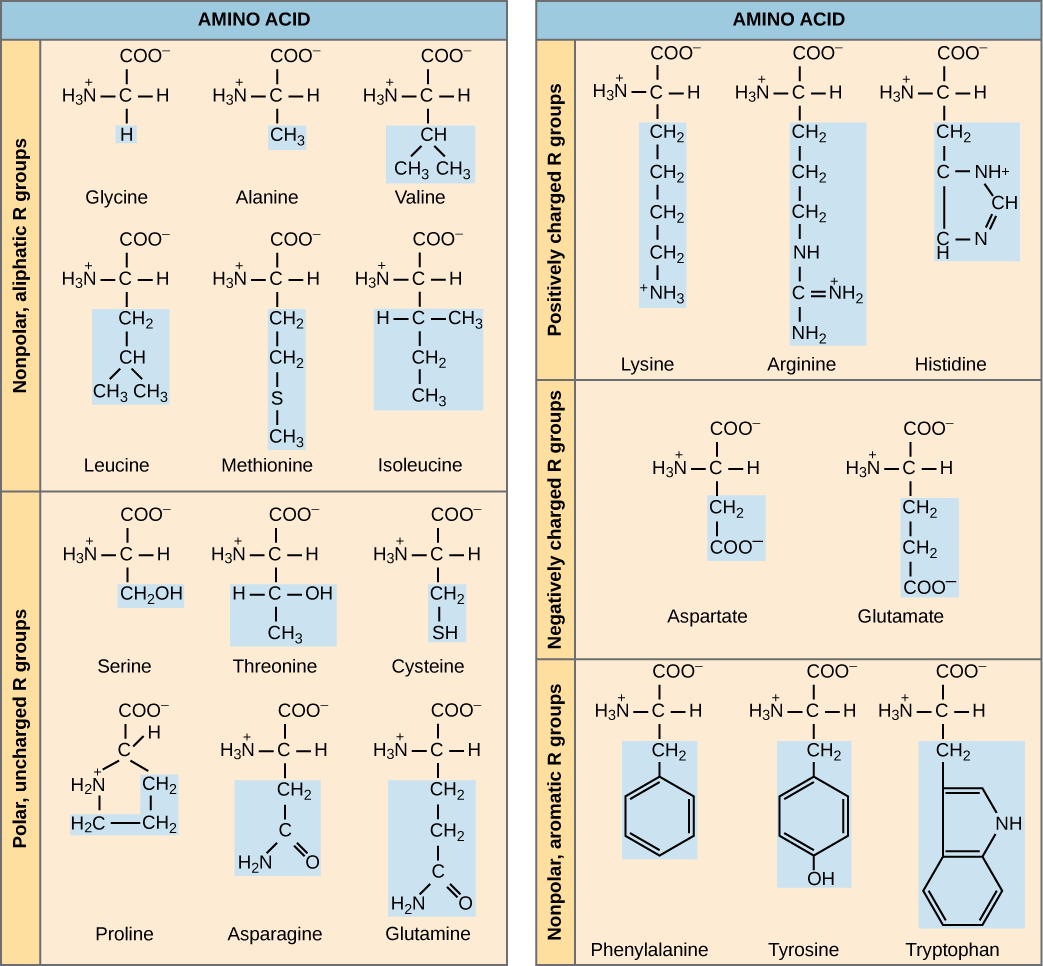
\includegraphics[width=0.8\textwidth]{aminoacids2.png}
  \caption{CAPTION AND REFERENCE}
  \label{fig:aminoacids}
\end{figure}

Two aminoacids are joined together through the formation of a peptidic (covalent) bond between them. Such a linkage is formed by removal of the elements of water (dehydration) from the $\alpha$-carboxyl group of one amino acid and the $\alpha$-amino group of another \cite{Nelson2008}. The remaining $\alpha$-amino and $\alpha$-carboxyl groups are available for linkage to other aminoacids, and in this way peptidic chains or peptides can be created.

While there are 20 basic units that constitute the majority of naturally observable proteins, their side chains can be modified both by physiological processes and by experimental procedures cite. One frequent instance of such modifications is the oxidation of methionine.


\section{The protein-focused biotechnology industry}


Proteins carry out most of the cell\textquotesingle s molecular functions, they work as molecular agents that can perform an extremely wide range of tasks. The advent of biotechnology has sought to take advantage of this power, either by using proteins as present in natural conditions (wild type) or engineered by humans. This potential economic activity is carried out by several biotech companies, including Novozymes A/S (NZ).

\ac{NZ} is a company whose line of business consists of the development of enzymatic products performing chemical transformations in different industrial processes. The application of these products, instead of conventional chemical-based solutions, has the advantage that they require less chemical substances, potentially simplifying industrial processes, reducing their costs and their environmental impact. Notorious examples of such applications include waste-water treatment, household care and the baking industry.


The advancement of the way \ac{NZ} does protein research is thus key to place the organization ahead of its competitors. The refinement of the currently used tools and the development of new ones could be of great significance for the company. 

Protein research can be approached from different angles. This thesis exploited the combination of mass spectrometry (\ac{MS}) and proteomics workflows (see chapter \ref{chap:mass_spec}) for the qualitative and quantitative characterization of protein samples.



\section{Objectives of the Thesis}
\label{sec:objectives}

In line with the goal of making \ac{NZ} more competitive, this project aimed at the following objectives:

\begin{enumerate}

\item Develop an open-source, Linux based and easily deployable pipeline for the analysis of \ac{MS} data, starting at the raw high-throughput data files and ending in the  biological interpretation of the results.

\item Evaluate this pipeline with a benchmark dataset to assess if the pipeline is able to reflect the biological phenomena captured in the data.

\item Establish a label-free quantification probabilistic model that provides relative abundance estimates and a measurement of their uncertainty based on the available data.

\end{enumerate}

\section{Structure of the Thesis}

An overview over the \ac{MS} and following computational data analysis steps is presented in \ref{chap:mass_spec}. The pipeline development and its benchmark are explained in chapters \ref{chap:pipeline} and \ref{chap:benchmark}, while the modelling problem is introduced in chapter \ref{chap:model}. Finally, a conclusion of the work is given in chapter \ref{chap:conclusion}.


\chapter{Mass spectrometry and shotgun proteomics overview}
\label{chap:mass_spec}

Life systems consist of complex systems, meaning their behaviour cannot be easily explained by analyzing the individual elements alone. Moreover, they present multiple layers of complexity, given by the nature of the elements that make it up. The layer provided by proteins is one of them, and its study is called proteomics. It is a complex layer because thousands of different proteins can be present in a single cell at any time, and their exact composition and quantities constantly change, responding to the stimuli of the surrounding environment. The study of the protein-specific complexity is called proteomics. With proteomics, one endeavors to infer the protein composition of a sample, and eventually quantify its protein amounts.

It may be useful to divide the existing approaches into two types of paradigms: top-down and bottom-up. In the top-down paradigm, intact proteins are directly used for the analysis. In the bottom-up paradigm, the proteins are first cleaved into smaller parts, and these parts are then used for identification, characterization, and quantification. These smaller parts are called peptides. \cite{Barsnes2008} CITE 1.6.1 COMPUTATIONAL METHODS. Such peptides acquire physicochemical properties fitting the requirements of the downstream analytical methods, mainly mass spectrometry (MS), which performs the data acquisition. The bottom-up paradigm is most often used because peptides are much more suitable to analysis by mass spectrometry, as explained in \ref{subsec:the_detector}. The top-down paradigm will be ignored in the rest of the manuscript.



MS is performed by means of a mass spectrometer, an ensemble of pieces of equipment that can acquire mass measurements for plenty of sample components. A detailed explanation of the sample processing required prior to MS is given in section \label{sec:sample processing}, while an overview on mass spectrometers is given in section \label{sec:the mass spectrometer}. The result of the MS analysis is a dataset that, with adequate computational analysis tools, is enough to perform the inference steps required to gather knowledge about the original protein sample. These inference steps can be condensed to the peptide and protein inference problems, explained in section \label{sec:peptide and protein inference}. A third computational problem needs to be solved if quantitative, and not just qualitative information, is to be gained from the experiment. This is the quantification problem, explained in section \label{sec:quantification} CITE.

A summary of the bottom-up approach MS analytical pipeline is provided in the rest of the chapter. It can be divided into two main steps:

\begin{enumerate}

\item \ac{MS} analysis and data generation. Sections \ref{sec:sample_processing} to \ref{sec:mass_spectrometry_workflows}.

\item Computational analysis of data. Sections \ref{sec:search_engines} to \ref{sec:quantification}.

\end{enumerate}


\section{Sample processing}
\label{sec:sample_processing}

An \ac{MS} experiment starts with the generation of protein mixture samples. They are first separated in order to sort the proteins via physicochemical criteria. This is most frequently carried out via SDS-PAGE based on mass or isoelectric point. Once the electrophoresis is completed, protein bands can be excised from the gel. Each band will contain a subset, or even only one of the proteins originally available, thus making the downstream analysis simpler \cite{Barsnes2008} REFERENCE COMPUTATIONAL METHODS CHAPTER 2

The reduced complexity protein mix is extracted in a denaturalized state so as to remove biases due to the divergent properties acquired by folded proteins. Then, proteins are subjected to digestion with specific enzymes, that can cut the aminoacidic chains following a predictable pattern. Trypsin is the most frequently used for this task, which cuts peptidic bonds whenever a positively charged residue, either Lysine (K) or Arginine (R), lies on the carboxyl side of the peptidic bond. Even though enzymes are very specific, the cleaving process is far from perfect, as there could be: \cite{Barsnes2008} COMPUTATIONAL METHODS 3.2

\begin{enumerate}

\item Missed cleavages \label{item:missed_cleavages}

\item Unsuspected cleavages during the maturation/life cycle of the protein.

\item Unexpected cleavages occurring either in the wet-lab procedure of the proteolytic treatment.

\item Naturally occurring, intentionally or unintentionally induced chemical modifications.

\end{enumerate}

\Cref{item:missed_cleavages} can happen due to steric inaccesability or the presence of specific aminoacids that can weaken the enzyme\textquotesingle s function. This is the case of Trypsin whenever the residue on the other side of the peptidic bond is Proline. This variability, though limited, needs to be taken care of in downstream analysis, as it could introduce biases in peptide observability. The other 

The result of this process is a mix of peptides following a length distribution given by the cleavage sites frequency and each protein\textquotesingle s aminoacidic composition. For Trypsin, the average peptide length is 10 residues, as roughly 1/10 residues are either R or K.
As explained in \ref{subsec:the_detector}, this length distribution is fitted to the resolution of the MS analyzer, thus optimizing the throughput of the method. An overview over mass spectrometers follows.

\section{The mass spectrometer}
\label{sec:the_mass_spectrometer}

The mass spectrometer consists of three main parts: an ion source, a mass analyzer, and a detector (see figure \ref{fig:mass_spectrometer}).

\begin{figure}[!h]
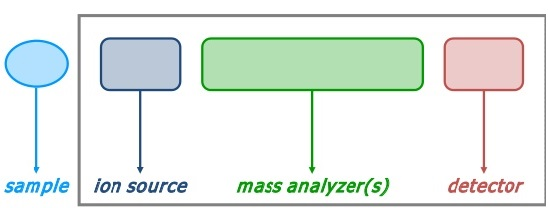
\includegraphics[width=\textwidth]{mass_spectrometer}
\caption[]{Schematic view of a mass spectrometer. Taken from \footnotemark}
\label{fig:mass_spectrometer}
\end{figure}

\footnotetext{\href{https://www.slideshare.net/joachimjacob/bits-introduction-to-mass-spec-data-generation}{https://www.slideshare.net/joachimjacob/bits-introduction-to-mass-spec-data-generation}}

\subsection{The ion source}
\label{subsec:the_ion_source}

All mass spectrometers exploit the physical properties of mass and electric charge exhibited by the analyzed components. Ionization of the analytes is absolutely essential prior to any measurement, as analytes left uncharged will be unobservable to the equipment.
This step is performed in the ion source \cite{Barsnes2008} CITE 5.1 COMPUTATIONAL METHODS. The most frequent ionization methods in proteomics are Matrix-Assisted Laser Desorption-Ionization (MALDI) and Electro Spray Ionization (ESI) CITE. Most peptides ionized by MALDI will acquire a single charge, whereas ESI can provide multiple charges (+2, +3, etc) too. Thus, the charge exhibited by an ion is not obvious when produced via ESI. Moreover, ESI can be run online with the right robotic equipment, while MALDI demands waiting time for vacuum generation. Finally, due to the chemical nature of the matrix components, MALDI ionizes more easily peptides containing aminoacids featuring aromatic rings (PYW), thus introducing a bias. Bias in ESI is less predictable. This is known as the competitive ionization problem. REF ALL THIS

The acquired charge yields a mass/charge (\ac{m/z}) ratio, a property that can be applied in the downstream component separation and measurement steps.

\subsection{The mass analyzer}
\label{subsec:the_mass_analyzer}

The plethora of ion separation methods is reflected upon the range of different analyzers available, mainly time of flight (\ac{TOF}), Ion trap (\ac{IT}) and quadrupole (\ac{Q}). These apply different principles to perform the same task: separation (analysis) of the ion mix by the \ac{m/z} ratio.

Moreover, two other analyzers exist which combine mass analysis with intensity measurement. These are Fourier Transform Ion Cyclotron Resonance (\ac{FT-ICR}) and Orbitrap. They both register cylotron resonance frequencies that are Fourier transformed into the spectrum space. Remarkably, \ac{FT-ICR} exhibits great resolving power, at the cost of high maintenance costs and difficult operability. 

\subsection{The detector}
\label{subsec:the_detector}

Detectors measure the intensity of an incoming ion signal. The ion\textquotesingle s \ac{m/z} ratio is known thanks to the previous mass analysis step. Performed for enough \ac{m/z} ratios, the detector can produce a \ac{MS} spectrum, which shows the intensity of ion current over an \ac{m/z} range. Some topics in signal detection in \ac{MS} need to be discussed.

On the one hand, the precision of the signal measurement is given by its mass resolution It is conventionally defined as the closest distinguishable separation between two peaks of equal height and width \cite{Marshall2013}. The resolution decreases as the \ac{m/z} ratio increases because small increments in the \ac{m/z} ratio become negligible at high \ac{m/z} ratios. This is one of the reasons why proteins are better fit for analysis when digested into peptides, as \ac{m/z} are reduced, thus increasing the mass resolution.

On the other hand, due to the natural occurrence of isotopes, particularly \ce{^{13}_{}C}, the same peptide will induce the measurement of several signals with very close \ac{m/z} values. They constitute the isotopic envelope of the ion SEE FIGURE, and represent the signal created by peptides containing an increasing number of \ce{^{13}_{}C} atoms. Every time a \ce{^{12}_{}C} is replaced by \ce{^{13}_{}C}, the mass increases by 1 Da. Even though the natural abundance of \ce{^{13}_{}C} is 1.1 \%, the sheer number of carbon atoms in a peptide makes it likely that at least one or even more carbon atoms will be \ce{^{13}_{}C}, eventually driving the pure \ce{^{12}_{}C} signal to comparatively small intensity values, and down to intensities below the background noise. Such event can be problematic if it entails that the \ce{^{13}_{}C} peak is confused for the \ce{^{12}_{}C} peak.

The resolution achieved by modern equipment allows for the distinction of each individual signal in most isotopic envelopes. Remarkably, the separation across peaks in the envelope can be used to infer the charge of the peptide, as increases of 1 Da at charge 1 will induce a separation of 1 \ac{m/z}, while at charge 2 it will be $1/2 = 0.5$ \ac{m/z}, at 3 $1/3 = 0.33$ \ac{m/z}, and so on.

It is up to the \ac{MS} technician to decide on the best pieces of equipment according to their availability and particularities of the dataset.

\section{Mass spectrometry workflows}
\label{sec:mass_spectrometry_workflows}

The \ac{MS} workflow diverges based on the simplicity of the original protein sample. When it consisted of a single protein, Peptide Mass Fingerprinting (PMF) is used, otherwise tandem MS (MS/MS) shall be performed. 

\subsection{Peptide Mass Fingerprint (PMF)}
\label{subsec:pmf}

If the original sample was known to contain a single protein, PMF, or \textit{protein-centric} proteomics, is conducted. In PMF, the mixture of peptides can be already transferred to the spectrometer, where a spectrum containing a peak for every m/z ratio present in the ionized peptide mix will be recorded. The resulting spectra can be considered a pattern, or fingerprint, of the peptides making up the original protein, thus enabling the identification of the original protein.


\subsection{High pressure liquid chromatography-Tandem MS}
\label{subsec:ms2}

\subsubsection{High pressure liquid chromatography (HPLC)}

If presented with the problem of analyzing a mixture of proteins, the capacities of mass spectrometers are easily overwhelmed by a too complex mixture, resulting in the analysis of only a minor part of the total protein  of the sample. This can be surmounted by splitting the initial sample into fractions, and using a series, or tandem, of spectrometers in the analysis. The spectrometers are used to analyze each obtained fraction separately, using different schemes.

Fractionation is achieved by different methods of separation CITE 1.7, most commonly via \ac{HPLC} methods, like reverse phase chromatography (separating on hydrophobicity) and strong cation exchange chromatography (separating on isoelectric point) \cite{Barsnes2008} CITE 4.2 computational methods.

\ac{HPLC} methods work by loading the peptide mix in a column containing a stationary and a solid phase. These phases create an environment where peptides interact differently based on their physico-chemical properties, set by the nature of the phases. The output of the column, called elute, will consist of subsets or fractions of peptides leaving the column at different retention times (\ac{RT}) i.e the amount of time passed before the peptide is observed in the mass spectrometer. Therefore, the input to the machine will consist of a simplified mix of peptides at a time. Notably, the same peptide could elute in several contiguous fractions.


\subsubsection{First MS analysis}

The tandem MS \ac{MS/MS}) analysis starts at the first \ac{MS} scan (\ac{MS1}), when the peptide mix accesses the analyzer. It is ionized in the ion source and enters the first mass spectrometer. While different ways of handling the peptides are available, we will focus on the product ion scan method. In this protocol, the first analyzer is used to select ionized peptides within a narrow m/z window.


\subsubsection{Fragmentation}
\label{subsubsec:fragmentation}

As the protein sample complexity increases, the \ac{MS1} information on the peptide fractions will not be enough to correctly map each to the original protein, thus rendering a correct interpretation of the resulting spectra impossible. Therefore, more information needs to be extracted from them.

Learning the peptide sequences would provide an additional feature that would make the peptide to protein mapping possible. This can be achieved by peptide fragmentation, which triggers the breakage of bonds along the peptidic chain, turning the peptides into smaller fragments. A given bond will be more likely to break the less stable it is. This makes (I) the \ce{C_$\alpha$}-\ce{CO}, (II) the peptidic \ce{CO}-\ce{NH}, and (III) the \ce{C_$\alpha$}-\ce{NH} bonds the more likely to break (see figure \ref{fig:abcxyz}). A nomenclature REF was introduced to name these fragments:

\begin{figure}[!h]
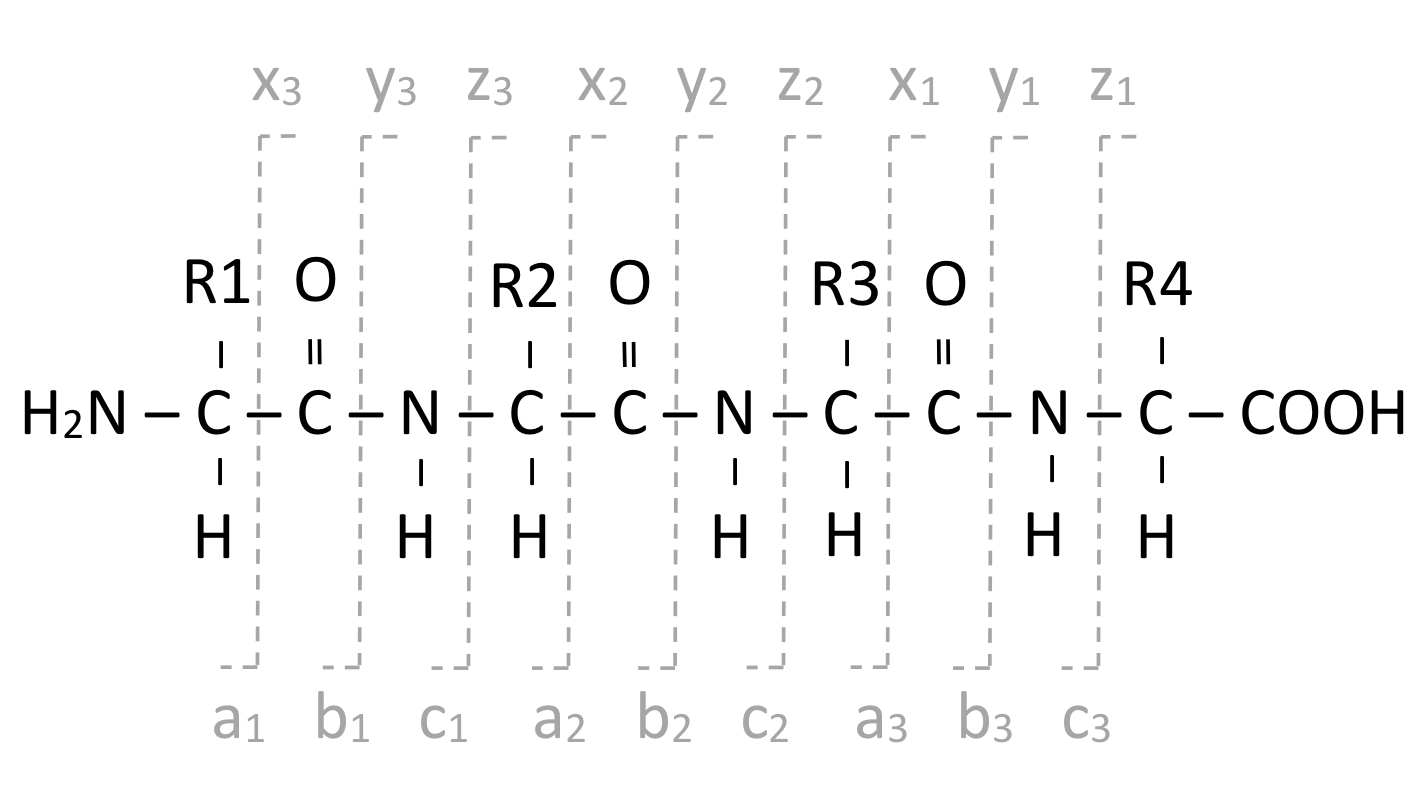
\includegraphics[width=\textwidth]{abcxyz}
\caption{The common fragments and their relation to the peptide sequence can be organized into 2 groups of 3 series each. The abc fragments keep the N-terminal residue, while xyz keep the C-terminal one. The a/x, b/y and c/z series are produced by the breakage of bonds I, II and III respectively. Specific fragmentation techniques make fragments belonging to one series more likely than others. Other fragments are possible but much less likely. Taken from CITE COMPOMICS TUTORIAL}
\label{fig:abcxyz}
\end{figure}

Provided enough mass resolution, the mass difference between contiguous fragments of the same series i.e a1 and a2, can be related to the mass of the extra residue in the longer fragment. If this comparison process is repeated for enough fragment pairs of the same peptide, a sequence can be read, finally providing sufficient information to perform an accurate peptide to protein mapping.

Fragmentation in proteomics is performed via (I) collision-induced (CID) or (II) electron-induced (EID) dissociation. CID is an ergodic fragmentation technique where peptides enter a collision cell containing an inert gas. Given enough kinetic energy, hits between ionized peptides and the gas will trigger the fragmentation of the peptide into smaller units. \cite{Barsnes2008} PAG 123 COMPUTATIONAL METHODS. Since the kinetic energy is randomly distributed across the peptide, the weakest bonds will break first. This results in the production of mostly b and y fragments, as well as the loss of any chemical modifications \cite{Barsnes2008} CITE pag 134 computational methods.

EID is produced by the hits against the molecule, which tend to occur on the areas of the peptide more positively charged. Thus, the fragmentation process is not ergodic and returns TYPE ions. More importantly, chemical modifications are not lost in the process.

\subsubsection{Second MS analysis}

The produced fragments enter the second analyzer \ac{MS2}, where a m/z spectrum of the fragments is recorded. Thus, unlike in PMF, where the spectrum recorded reflects the m/z ratios acquired by the protein peptides cleaved by the enzyme, tandem MS spectra on product ion scan mode record the m/z ratio of the fragments produced by an ionized peptide with a given m/z ratio. The m/z ratio of this precursor ion is changed during the run, thus, multiple spectra are obtained where PMF would create only one. The \ac{MS2} spectra will encode the sequence of each peptide as mentioned in \ref{subsubsec:fragmentation}, and with the right tools, it can be deconvoluted and interpreted as explained in \ref{sec:search_engines}.


\section{Spectra processing: search engines}
\label{sec:search_engines}

\ac{MS} search engines are capable of performing the peptide to spectrum matching (PSM). They do it by building statistical models that find the peptides within a protein database that best explain the observed spectra. \textit{De novo} search engines exist that don't require a reference proteome, but better results are obtained when using one..DEVELOP THAT.

Matching is possible by predicting the cleavage pattern of each protein sequence in the database \textit{in silico} based on the cleavage pattern of the enzyme used, coupled with the simulation of the expected spectrum based on the predicted peptides.

Given the stochastic nature of the protein cleavage and spectra recording processes, the resulting spectra exhibit variability manifested in missing peaks or spurious ones. Furthermore, random (wrong) matches can be returned by the PSM process when running against a sufficiently big database. This translates to the generation of multiple matches, of which one, if any, will be correct. Therefore, the lists of matches need to be somehow ranked. The issue is addressed by search engines through the deployment of statistical models that provide scoring systems measuring the goodness of the match. Assuming the correct protein is present in the database, a good scoring system should give the best score to the right peptide. Under this circumstances, if repeated for several peptides, enough evidence for the presence of individual proteins can be collected.

Multiple search engines exist that implement different matching and scoring algorithms. The most modern ones include MS-GF+, MS-Amanda, Comet, X!Tandem or Andromeda CITE THE ENGINES. Notably, the results of each individual search engine can be combined to gather their strengths, at the expense of an increased computational cost and time REF THIS!!



\section{Validation and quality control}
\label{sec:validation}

The scoring system implemented by search engines provides the best matches, but they are bound to contain false identifications. Nevertheless, these scores can be used to apply a filter that aims at minimizing the amount of errors.

A common filter is the false discovery rate (FDR), usually set to 1\%, indicating tha the application of this filter one out of a hundred filtered matches are expected to be false positives.

The most commonly used method to compute the FDR of a list of matches is the target-decoy search. Using this method, the search engine replicates the matching process, using the same spectra, but instead against a decoy database. This decoy database is generated by reversing or more generally applying a randomization technique upon the sequences present in the original database (target). This guarantess that while the sequences in the decoy database won't overlap with those in the target, their basic properties of the decoy (size, composition, etc) will remain identical to the target.

All matches to the decoy are by definition wrong. Since database properties 
are kept the same, the amount of matches to the decoy exhibiting less than a given score $s$ can be regarded as an estimate of the number of false identifications ($\hat{n}_{fp}$) in the equivalent list of target results. This is because the existence of shared properties entails that random matches are equally likely to happen in both databases CITE COMPOMICS TUTORIAL 1.5. Together with the number of PSMs passing a threshold score ($n_{tp} + n_{tp}$), the FDR can be computed using the formula below.

\begin{equation}\label{eq:fdr}
FDR = \frac{\hat{n}_{fp}}{n_{fp} + n_{tp}}
\end{equation}

Equation \ref{eq:fdr} can be used to select the number of positives (the denominator of the fraction) that make the FDR equal to a predefined value, frequently 0.01 or 1 \%.

%The minimal FDR at which a given PSM is considered a valid match constitutes the PSM\textquotesingle s q-value
%
%\begin{equation}\label{eq:qvalue}
%q(PSM_i) = \min FDR \forall PSM_i \in Positive
%\end{equation}

\section{Peptide and protein inference}
\label{sec:inference}

Two steps in protein identification can be distinguished:

\begin{enumerate}

\item \textbf{Peptide inference}: infer the peptides present in the sample.
\item \textbf{Protein inferece \textit{proper}}: based on the inferred peptides, infer what proteins generated them. This is not trivial as peptides are degenerate and could map to more than one protein.
\end{enumerate}

Peptide inference is performed during the PSM process. The ensemble of proteins most likely to have generated the list of peptides stemming from the filtered PSMs can be inferred using different algorithms. The degenerate nature of peptides is dealt with the Occam\textquotesingle s razor principle, which states that the most likely solution is the simplest one. Thus, protein inference algorithms aim at explaining the maximum amount of peptides using the least amount of proteins.

\section{Protein quantification}
\label{sec:quantification}

The combination of all the aforementioned computational analyses yields a list of protein identities that reports the protein composition i.e qualitative information of the original sample. However, in most proteomics applications, quantitative data can be of great interest, as many biological phenomena are manifested mainly through changes in the protein abundances, rather than protein presence alone. For instance, cancer cells in response to a drug could modulate the abundance of several proteins without removing them from the cytosol or introducing new ones.

Protein quantification pipelines can be classified based on whether isobaric labelling was used (label-based) or not (label-free). These are explained in subsection \ref{subsec:labelling}. If the label-free approach is employed, more distinctions can be made based on:

\begin{itemize}
\item The proxy used for quantification: spectral counting (\ac{SC}) or extracted ion currents (\ac{XIC}). These are explained in \ref{subsec:scvsxic}


\item The way the data are brought to the protein level from the peptide level: summarization-based vs. peptide-based.
\end{itemize}

\subsection{Label-based and label-free approaches}
\label{subsec:labelling}

Two paradigms exist in protein quantification: label-based and label-free. In label-based quantification, originally identical peptides from a number of different samples are made distinguishable by their masses via the incorporation of a label. All label-based methods simultaneously analyze several samples in each experiment, removing the difficulties associated with between-run variability \cite{Barsnes2008} CITE PAGE 237 COMPUTATIONAL METHODS The finite number of "plexes" available for a given label sets the limit to how many samples can be differentially quantified \cite{Cox2014}. Different techniques, like Stable Isotope Labeling by Amino acids in Cell culture (SILAC) CITE or Isotope-Coded Affinity Tags (ICAT) CITE, differ in the nature of the label and the way it is introduced. Remarkably, peptide labeling costs can be quite high. This, together with the limited amount of samples that can be compared makes a case for label-free quantification.

In the label-free quantification approach, peptides from different samples are not labelled differently and are thus distinguished by their presence in different, independent \ac{MS} runs. In order to account for inter-run variability in peptide identifications and \ac{RT}, a match-between-runs (MBR) processing can be carried out for pair-wise transfer of peptide identities from runs where identification was successful to those were it wasn't due to the randomness in the identification process. The transfer can be made based on shared precursor mass and corrected retention times CITE MOFF. Furthermore, in order to collect consistent \ac{XIC}, a feature extraction step can be  executed to extract the apex intensity of the identified peak clusters \ref{figure:moff}.


\begin{figure}[!h]
\centering
\begin{subfigure}{.45\textwidth}
    \caption*{A}
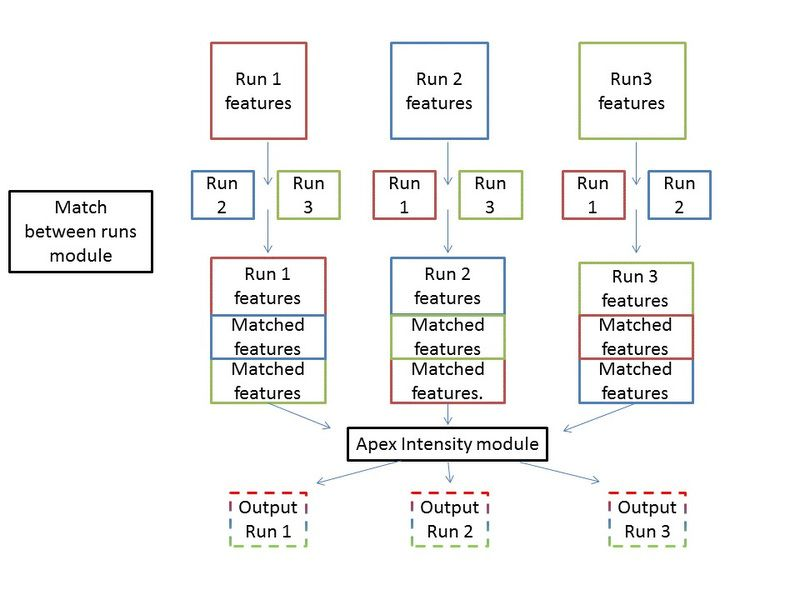
\includegraphics[width=0.9\linewidth]{moff_workflow}
\end{subfigure}
\begin{subfigure}{.45\textwidth}
    \caption*{B}
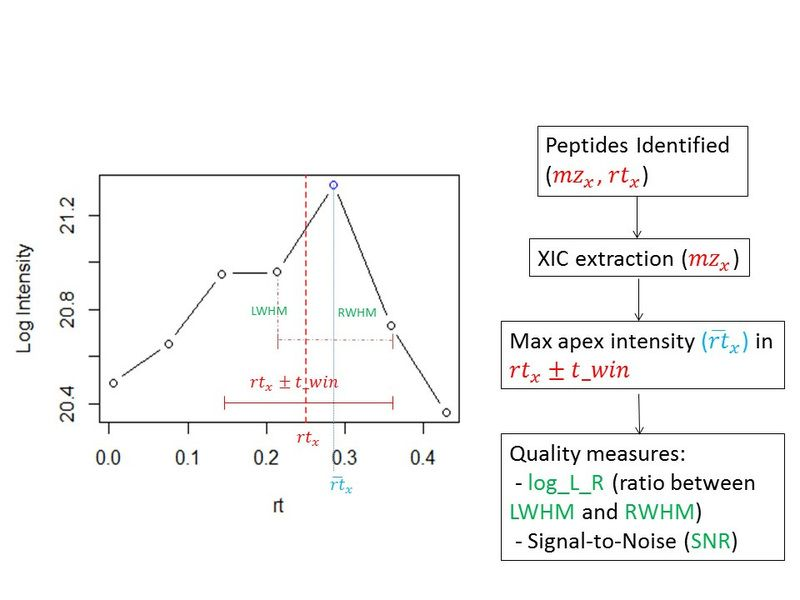
\includegraphics[width=0.9\linewidth]{apex_intensity}
\end{subfigure}
\caption{Illustration of the \ac{MBR} and apex intensity extraction steps. \textbf{A} the information gathered from matches in replicate runs is collected for a reanalysis of the spectra. \textbf{B} A retention time window can be used to screen the peak clusters and highest \ac{MS1} intensity of a peak cluster (apex intensity). Taken from CITE MOFF}
\label{figure:moff}
\end{figure}


\subsection{SC and XIC based quantification}
\label{subsec:scvsxic}


Quantification can be spectral counting or \ac{XIC} based.
Spectrum counting based quantification is the simplest quantification method in proteomics. It relies on the rationale that highly abundant peptides will have a higher intensity and are thus more likely to trigger the acquisition of MS/MS spectra. As a result, peptides from abundant proteins are more likely to be identified and in more spectra. Two approaches were hence followed: count the number of peptides identified for a given protein – like in the emPAI index method – or count the number of spectra ascribed to a protein as in the NSAF method CITE COMPOMICS 4.1. These methods have the advantage that they are very simple to implement and don't require any further data processing.

\ac{XIC} based methods rely on intensity measurements at any level of the \ac{MS} workflow as proxies for protein abundance CITE. A wide range of algorithms are available to process these data and output estimates of protein abundance. All of them require an intensive preprocessing step, usually including (I) taking the $log_2$ intensity to make the data distributions symmetrical and thus make it fit for diverse parametric tests, and (II) quantile normalization to address between-runs variability in the intensity measurements. They can be classified in the bases of which MS level is used as proxy for the protein abundances and on whether or not a summarization step is performed to aggregate peptide-level data into protein-level data, or not. 


Although the abundance of proteins and the probability of their peptides being selected for \ac{MS/MS} sequencing are correlated to some extent, \ac{XIC}-based methods should clearly be superior to spectral counting given sufficient resolution and optimal algorithms. These advantages are most prominent for low-intensity protein/peptide species, for which a continuous intensity readout is more information-rich than discrete counts of spectra. \cite{Cox2014} For this reason, only the \ac{XIC} approach will be regarded in the rest of the manuscript.  


\subsection{\ac{XIC}-peptide-based models for label-free quantification}
\label{subsec:peptide_model}

The data collected in the mass spectrometer refers to peptides originating from a latent protein composition, given by the original sample. However, the data interpretation requires the transfer of these peptide-level data into the protein level. This can be done by either (I) performing an aggregation of the peptide-level data, where a summary value of the peptide-level data is taken as representative for the protein-level data, or (II) performing the protein quantification directly at the peptide-level by means of linear regression models.

As stated in \cite{Goeminne2015}. \textit{Peptides originating from the same protein can indeed be considered technical replicates and theoretically should lead to similar abundance estimates. However, the summarization of the peptide intensities into protein expression values is cumbersome, and most summarization-based methods do not correct for differences in peptide characteristics or for the between-sample differences in the number of peptides that are identified per protein. This might introduce bias and differences in uncertainty between the aggregated protein expression values, which are typically ignored in downstream data analysis steps}.

It is for this reason that peptide-based models offer the statistical framework required to learn as much from the data as possible. This translates into improved results when compared to the other aforementioned methods \cite{Goeminne2015}.
%CITE MAXQUANT
%
% The MaxLFQ algorithm, provided within the MaxQuant suite, is an \ac{MS1}, summarization method performing two optimisation steps to  


\chapter{A label-free quantification proteomics pipeline}
\label{chap:pipeline}


\section*{Summary}
A pipeline making use of the set of tools published by the Compomics  and StatOmics groups SearchGUI, PeptideShaker, moFF and MSqRob CITE THEM, was developed to support complete label-free protein quantification analyses using the most recent advances in the field with open-source software. The pipeline can be run on Linux computer clusters to perform (I) peptide to spectrum matching against a reference database, (II) quality control and filtering, (III) MBR and feature extraction, (IV) protein inference and (V) relative quantification. Its output can be passed to follow-up analyses in R or Python to get a biological interpretation of the results.  A benchmark of its performance was accomplished using the proteome benchmark dataset published in \cite{Cox2014}. The results exhibited an accuracy similar to those achieved by the MaxLFQ \cite{Cox2014} software, excepting a bias produced by the sample fractionation of this dataset.


\section{Introduction}

\begin{figure}[!h]
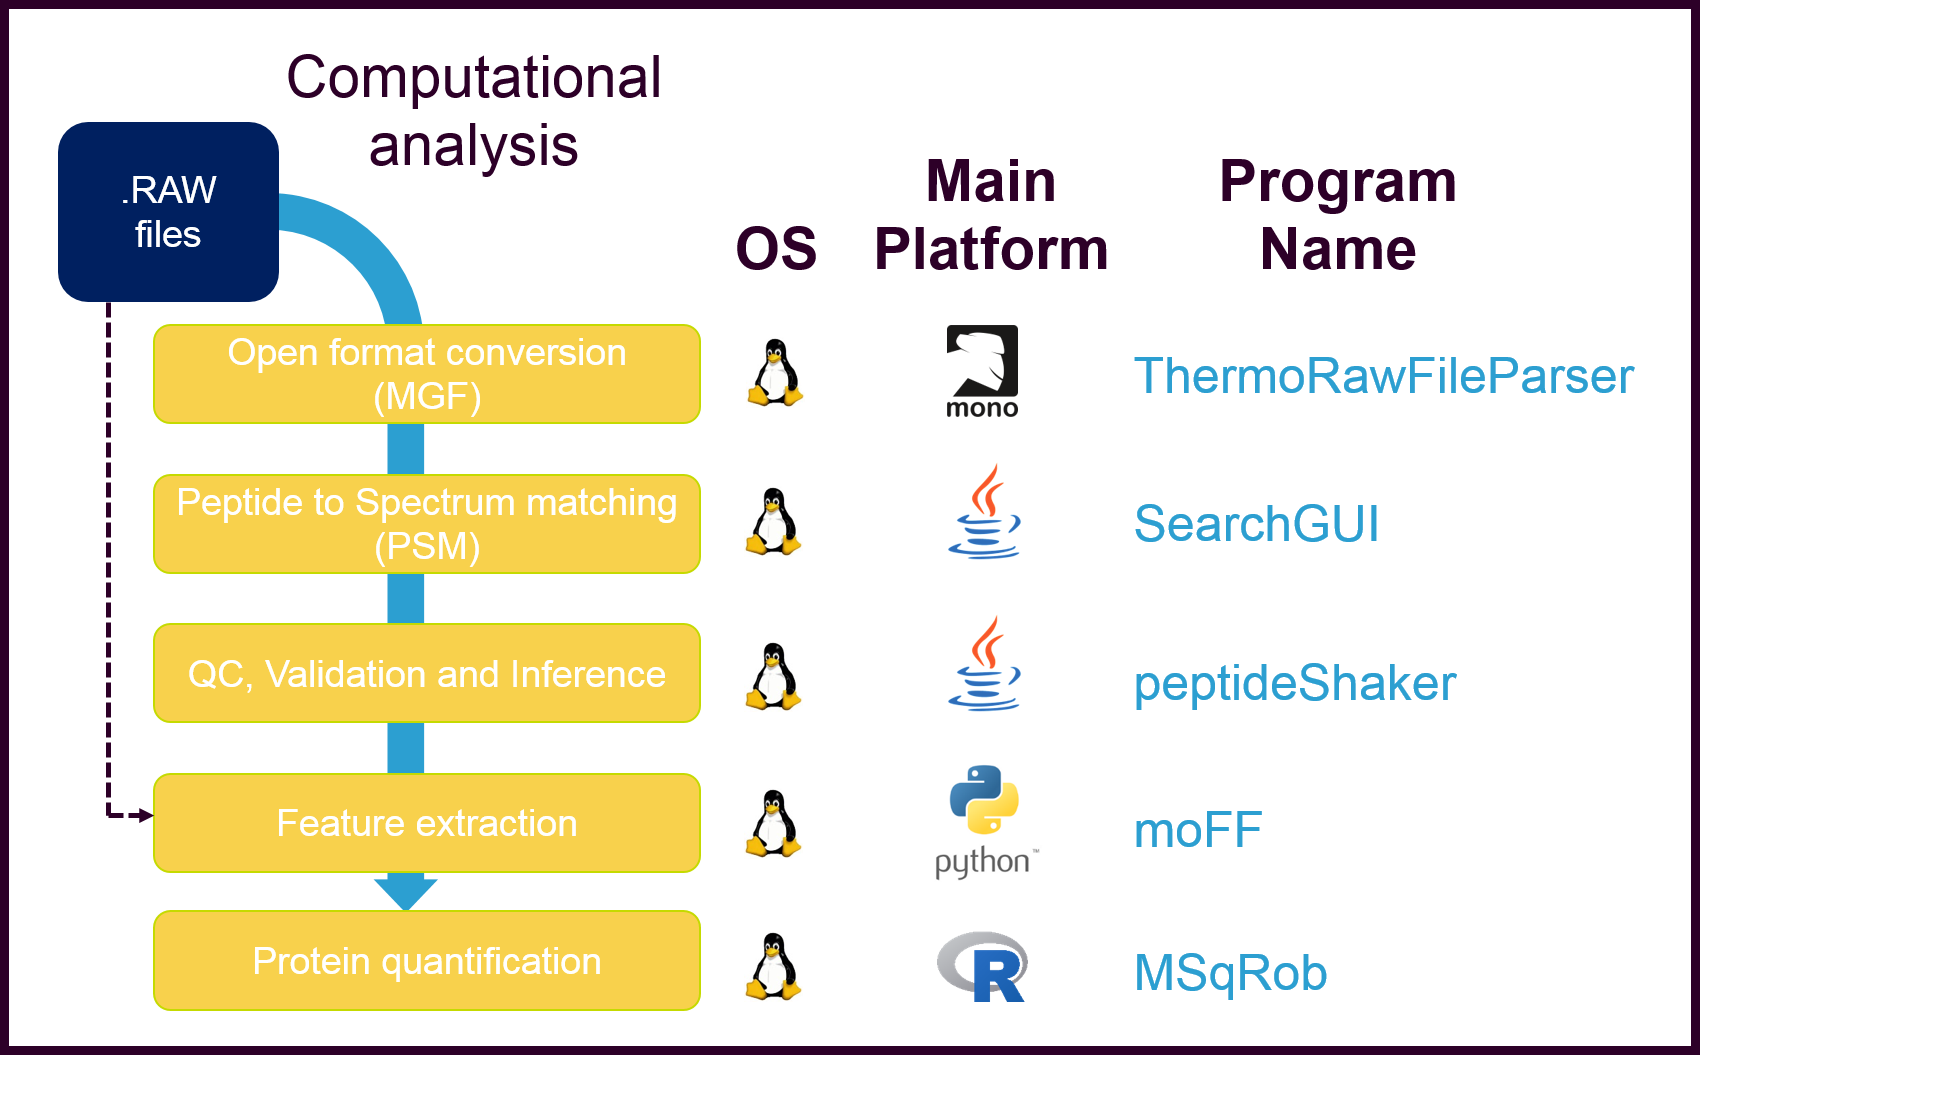
\includegraphics[width=\textwidth]{pipeline}
\caption{Pipeline}
\label{fig:pipeline}
\end{figure}


Several proteomics pipelines are available on the internet under different licensing conditions. Many are released as closed-source software, where information on how the program works is kept from the user. This is a serious drawback as it hinders the study of the implemented models and its customisation. Open-source, free alternatives, like the Trans Proteomic Pipeline (\ac{TPP}) or openMS  CITE ALL are nevertheless available for the community. MaxQuant, a free but closed-source proteomics analysis suite CITE MAXQUANT, has been extremely successfully adopted by the scientific community due to its ease of use and a comprehensive pipeline.

However, still only few of these tools have a fully Linux-supported, well-documented, command-line version available, which would make customised, automatic streamline analyses much easier to perform. As a GUI would not be required to run the pipeline, it would also be scalable to big datasets. Finally, having free licenses would imply that anyone, provided the technical knowledge, can perform the computational analysis independently, thus speeding the data to knowledge turnover in \ac{NZ} or any organization making use of it.

The development of a pipeline achieving these goals will be described in this chapter.

\section{Materials and Methods}

\subsection{Data generation and loading}

The proteome benchmark dataset from \cite{Cox2014} was reanalysed starting at the output RAW files available at the PRIDE repository \footnote{\href{https://www.ebi.ac.uk/pride/archive/projects/PXD000279}{https://www.ebi.ac.uk/pride/archive/projects/PXD000279}}. Briefly, the \textit{Homo sapiens} and \textit{E. coli (strain K12)} proteomes were mixed in 1:1 (condition L) and 1:3 (condition H) proportions, with 3 replicates for each combination. Moreover, each of the 3 replicates of the 2 conditions was analysed over 24 fractions. This experimental setting thus generated a total of $2 \times 3 \times 24=144$ RAW files. One file was missing in the repository. The ThermoRawFileParser CITE THERMORAWFILEPARSER program was used to convert RAW files to the open format MGF (Mascot Generic Format).

\subsection{Decoy database preparation and search}

The spectra saved in the MGF files obtained in the previous step were passed to the MS-GF+ search engine CITE by means of the SearchGUI \texttt{SearchCLI} tool CITE utility. The search parameters were set using the \texttt{IdentificationParametersCLI}. In order to account for potential post-translational modifications, the search was conducted allowing for the following variable modifications: oxidation of M and deamidation of N and Q. Moreover, C carbamidomethylation was set as fixed modification. The enzyme was set to semispecific Trypsin, allowing for a non-tryptic cleavage on any side of the peptide. Up to two missed cleavages were allowed. The precursor tolerance was 10 ppm and the fragment tolerance 0.5 Da. 


The target database was created by combining the Uniprot proteomes for \textit{E. coli (strain K12)} (UP000000625) and \textit{Homo sapiens} (UP000005640), downloaded in June 2018. The decoy database was created using the \texttt{FastaCLI} utility in SearchGUI by reversing all sequences in the target.

\subsection{Quality control and validation}

The SearchGUI results were filtered using the default built-in checks available in the PeptideShaker utility \texttt{PeptideShakerCLI} \footnote{\href{https://github.com/compomics/peptide-shaker/issues/300}{https://github.com/compomics/peptide-shaker/issues/300}}. By default, the FDR was set to 1\%. PEP and confidence statistics were computed using the PeptideShaker built-in algorithms. Output was extracted via the Default PSM report txt file, available in the \texttt{ReportCLI} utility.


\subsection{Data refinement}

The moFF command line utility CITE was applied to perform (I) match-between-runs and (II) extract MS1 apex intensity of each peak cluster. This required passing the original RAW files, together with the Default PSM report from PeptideShaker. Output was exported to a peptide summary file, containing  one row per peptide and for every peptide, the detected apex intensity in each sample.

\subsection{Quantification}

Relative quantification was performed using the MSqRob utility by passing the peptide summary file from moFF. Prior to quantification, the data was preprocessed using the \texttt{preprocess\_MSnSet()} function. In a nutshell, (I) MS1 apex intensities were $log_2$ transformed, (II) peptides belonging to protein groups that contained one or more proteins that were also present in a smaller protein group were discarded CITE MAIN MSQROB, and (III) protein groups with only 1 peptide were dropped. Intensity normalisation was not performed as a systematic bias in intensities is indeed expected for all \textit{E. coli} peptides from samples where the \textit{E. coli}proteome was 3 times more abundant.


Once preprocessing is done, a ridge regression model with Huber weights and empirical Bayes estimation of the protein variance was fit to every protein individually. The significance of the treatment effect differences was assessed through a Student\textquotesingle s T test, implemented in the \texttt{test.contrast()} function.

\subsection{Code implementation}

\section{Results}

\subsection{Peptide to spectrum matching step identified thousands of spectra}

The preprocessing of the RAW files produced by the mass spectrometer into the MGF open format enabled searchGUI to dispose of the registered spectra. PeptideShaker quality control and filtering capabilities (see figure \ref{figure:qc_validation}) carried out the required search results validation. As expected, matches to the target and decoy exhibited similar score distributions at low score values, while a divergence is observed at higher score values. Likewise, the m/z error was found to be closer to 0 on validated PSMs than on those which did not pass the 1 \% FDR filter. The application of this filter implied that the FNR (false negative rate) was set to 5 \%, i.e 5 out of every 100 discarded matches were estimated to be true positives.



\begin{figure}[!h]
\centering
\begin{subfigure}{.45\textwidth}
  \centering
  \caption*{A}
  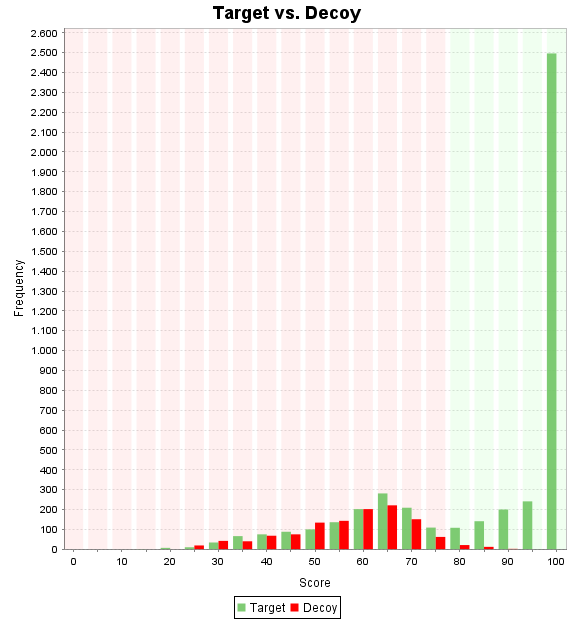
\includegraphics[width=.9\linewidth]{target_vs_decoy}
\end{subfigure}
\begin{subfigure}{.45\textwidth}
  \centering
    \caption*{B}
  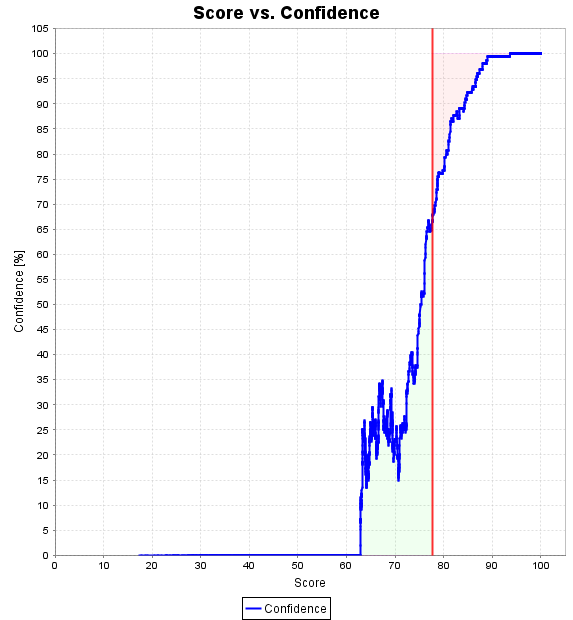
\includegraphics[width=.9\linewidth]{score_vs_confidence}
\end{subfigure}
\bigskip

\begin{subfigure}{.45\textwidth}
  \centering
    \caption*{C}
  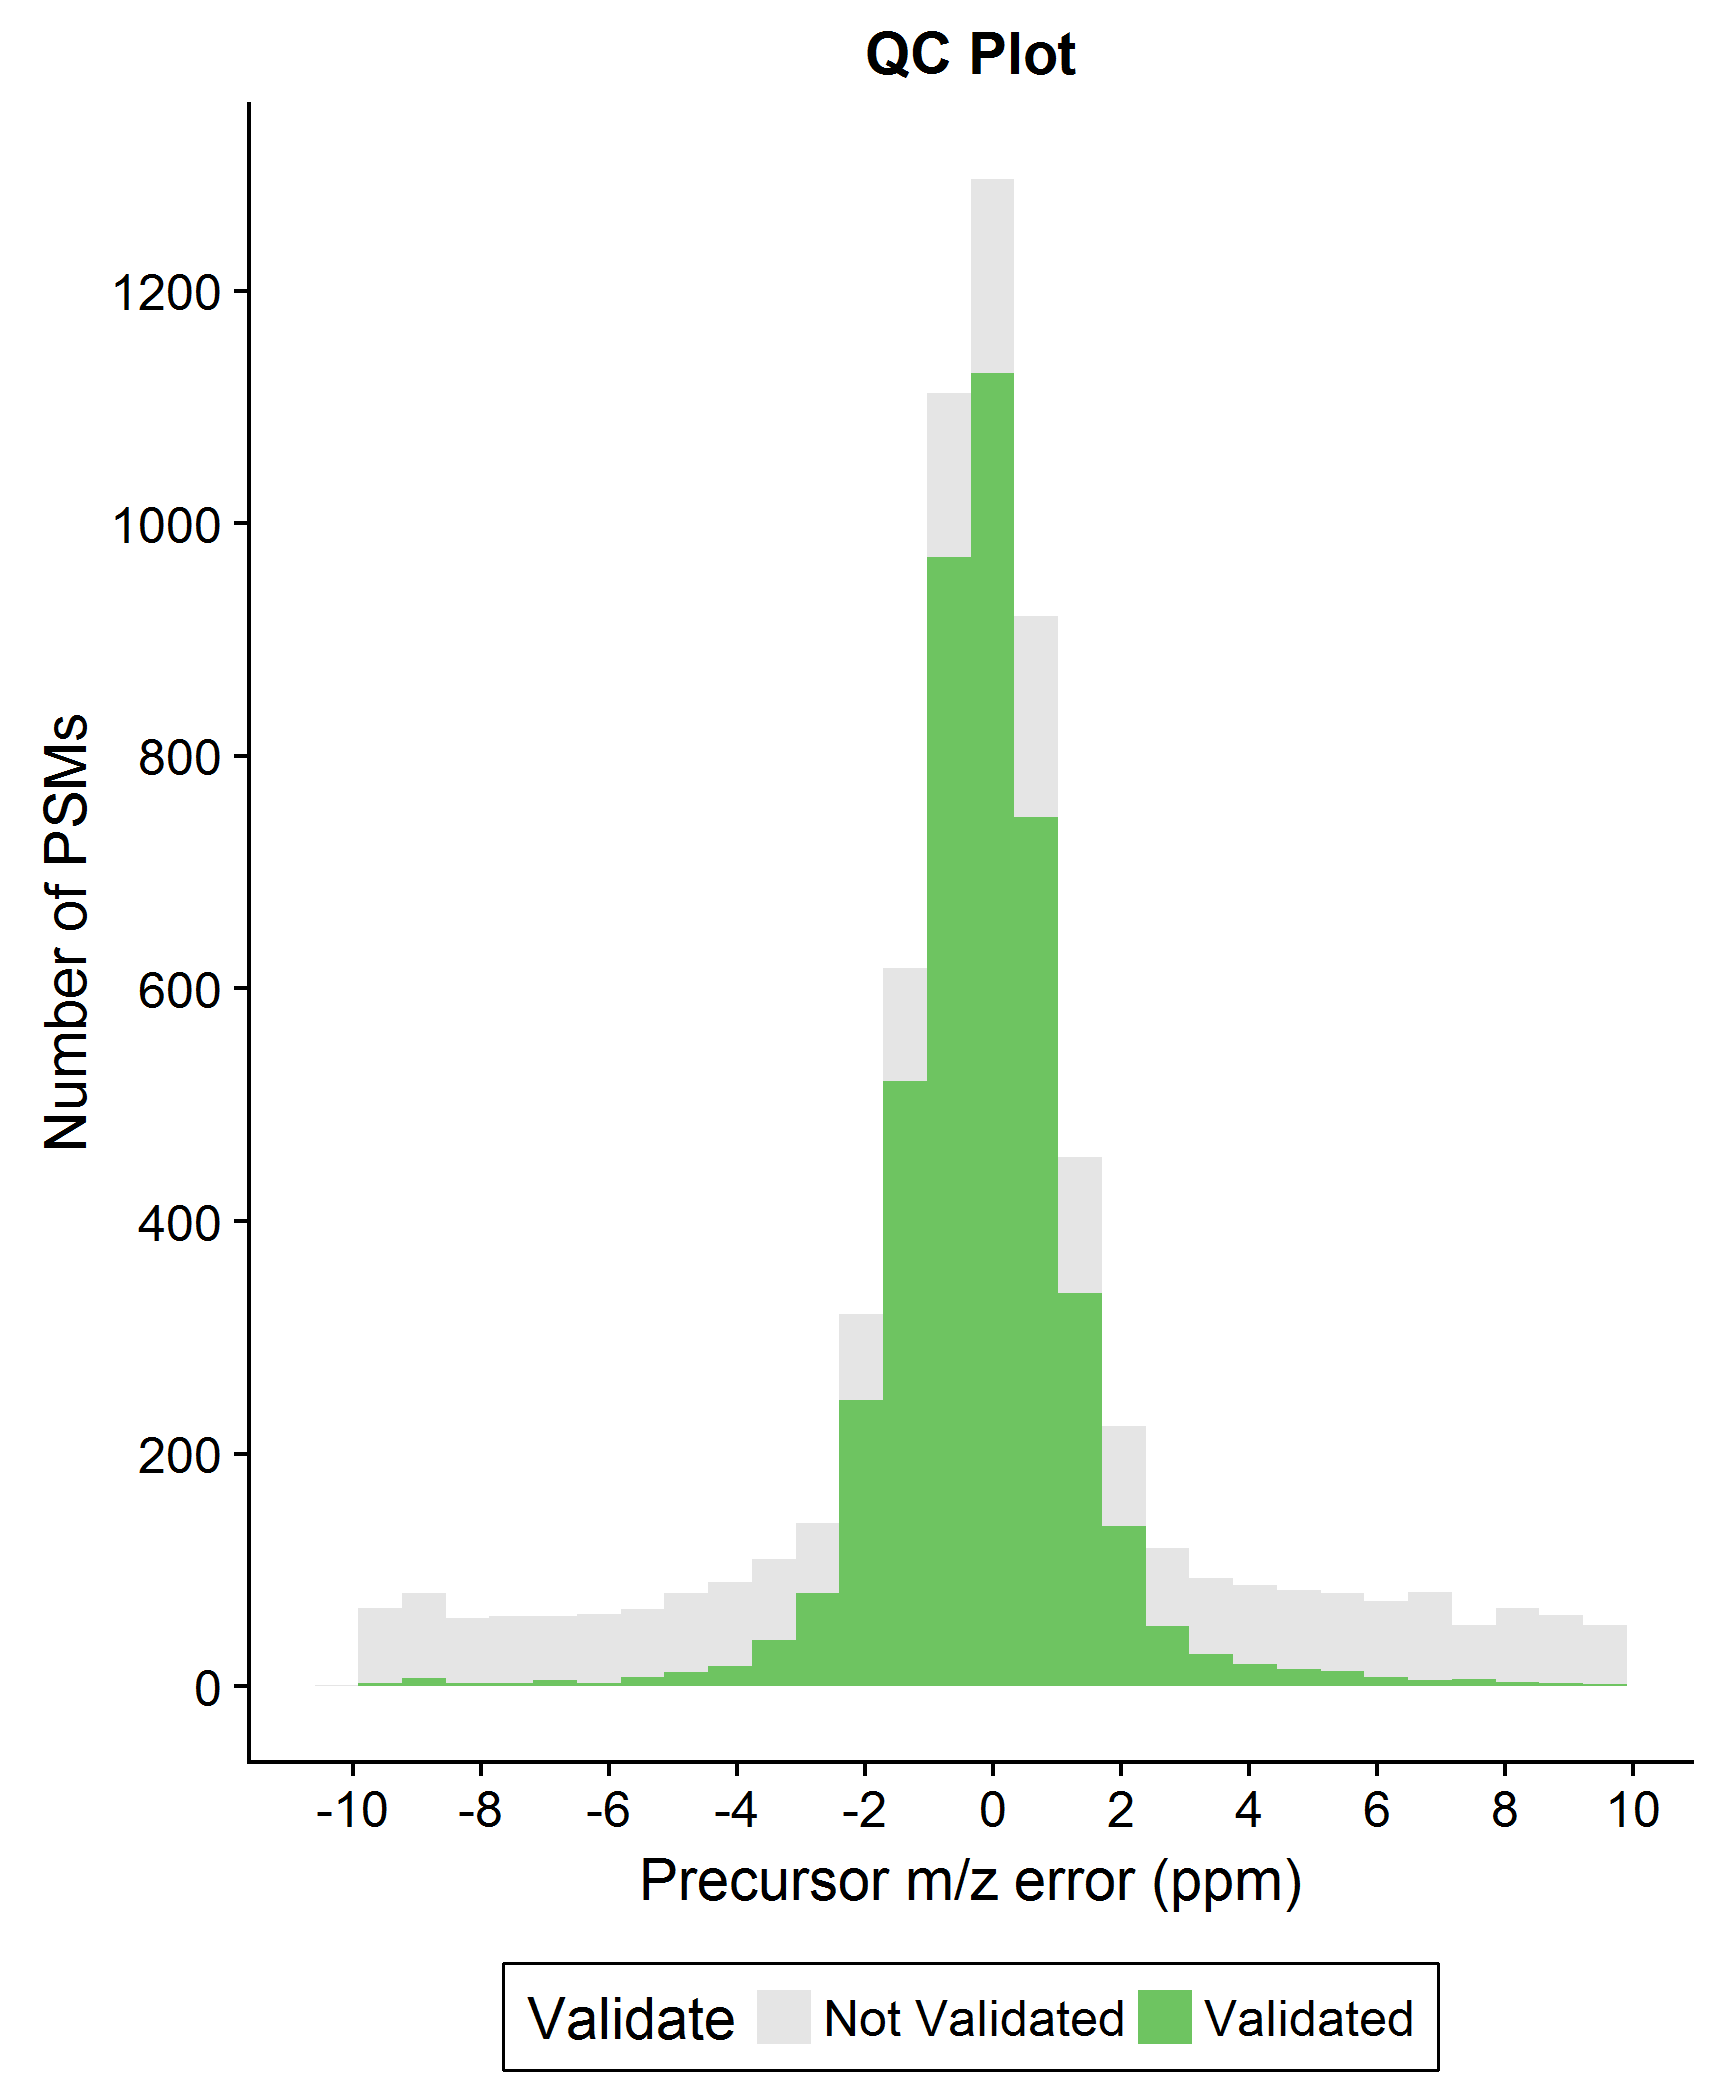
\includegraphics[width=.8\linewidth]{qc}
\end{subfigure}
\begin{subfigure}{.45\textwidth}
  \centering
    \caption*{D}
  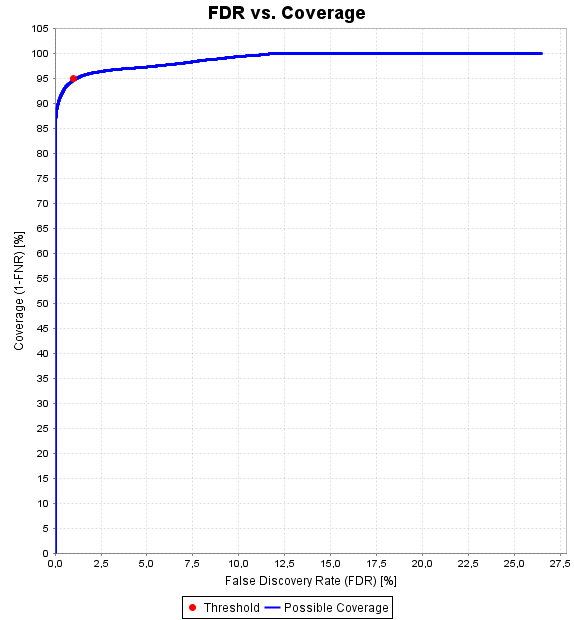
\includegraphics[width=.9\linewidth]{roc}
\end{subfigure}
\caption{Quality control and validation of the 13th fraction of the third replicate in condition L. \textbf{A} Score distribution for matches to the decoy and the target databases. \textbf{B} Evolution of the PSM score with confidence. The implemented cutoff at FDR of 1 \% is displayed with a red vertical line. \textbf{C} Distribution of the difference between the predicted and measured \ac{m/z} values, segregated by validation status. \textbf{D} ROC curve built upon the number of false positives and negatives estimated from the decoy search. The cutoff is displayed as a red dot.}
\label{figure:qc_validation}
\end{figure}

The PSM confidence is defined as $1-PEP$, where PEP stands for the Posterior Error Probability. Also known as local FDR, the PEP is an estimate of the probability of a given PSM of being an incorrect assignment. Thus, the confidence is the probability of the PSM being a correct assigment CITE NEVINZKY. The 1\% FDR cutoff selected PSMs with a score higher than 78, which translated to a confidence of at least 65\%.


The combination of both programs enabled the identification and validation (matching) of thousands of spectra with high confidence in all samples . However, when compared to the total amount of spectra available, the percentage of matched spectra was on average 37.4\%, with a marked decrease starting at fraction 14 (see figure \ref{fig:match_percent}).

\begin{figure}[!h]
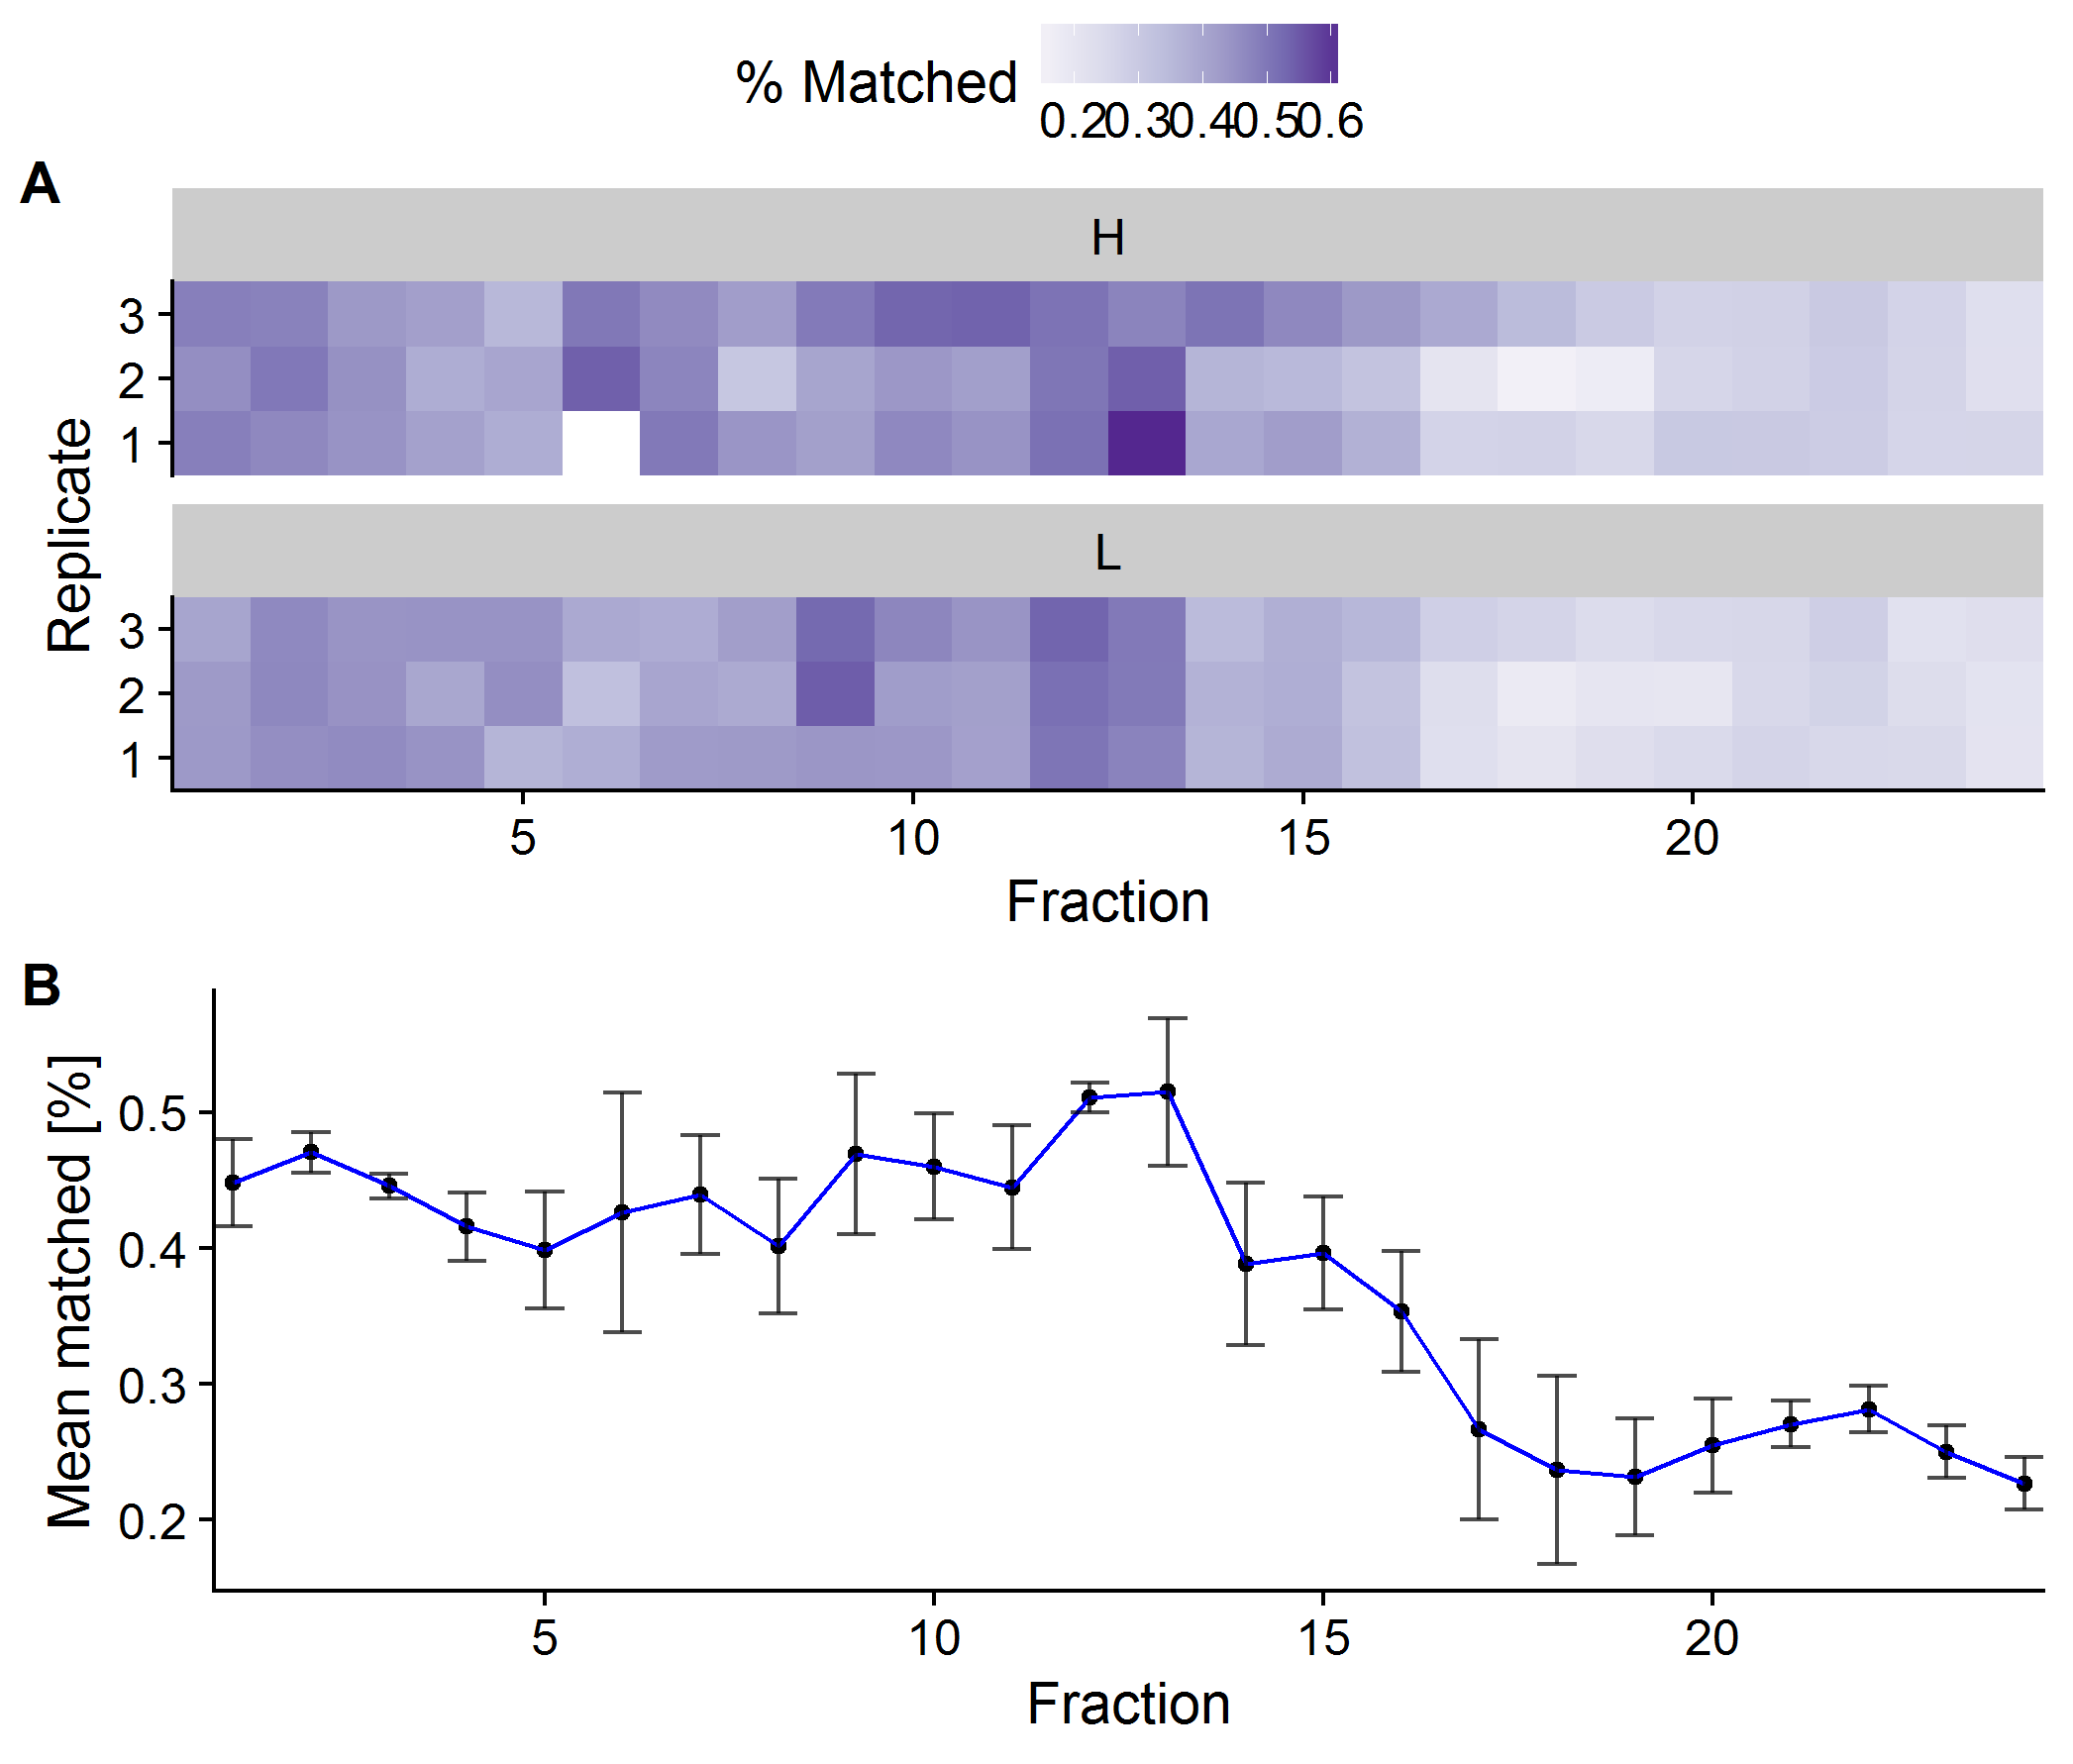
\includegraphics[width=0.8\textwidth]{match_percent}
\caption{Percentage of matched spectra in all samples. The total number of spectra per sample ranged between 5894 and 20249. \textbf{A} Percentages are encoded with a blue palette, the darker, the higher, and viceversa. \textbf{B} The mean for each analysed fraction across conditions and replicates is displayed together with error bars to represent the standard deviation. The sixth fraction of the first replicate in condition H was missing in the PRIDE data repository.}
\label{fig:match_percent}
\end{figure}


\newpage

\subsection{MBR and Apex intensity extraction capacitate for accurate quantification}

The match between runs step allows for increased identifications by transferring successful matches between replicate runs. The results of this process for the 13th fraction of the L condition is shown in figures \ref{fig:mbr_summary} and \ref{fig:mbr})

\begin{figure}[!h]
\centering
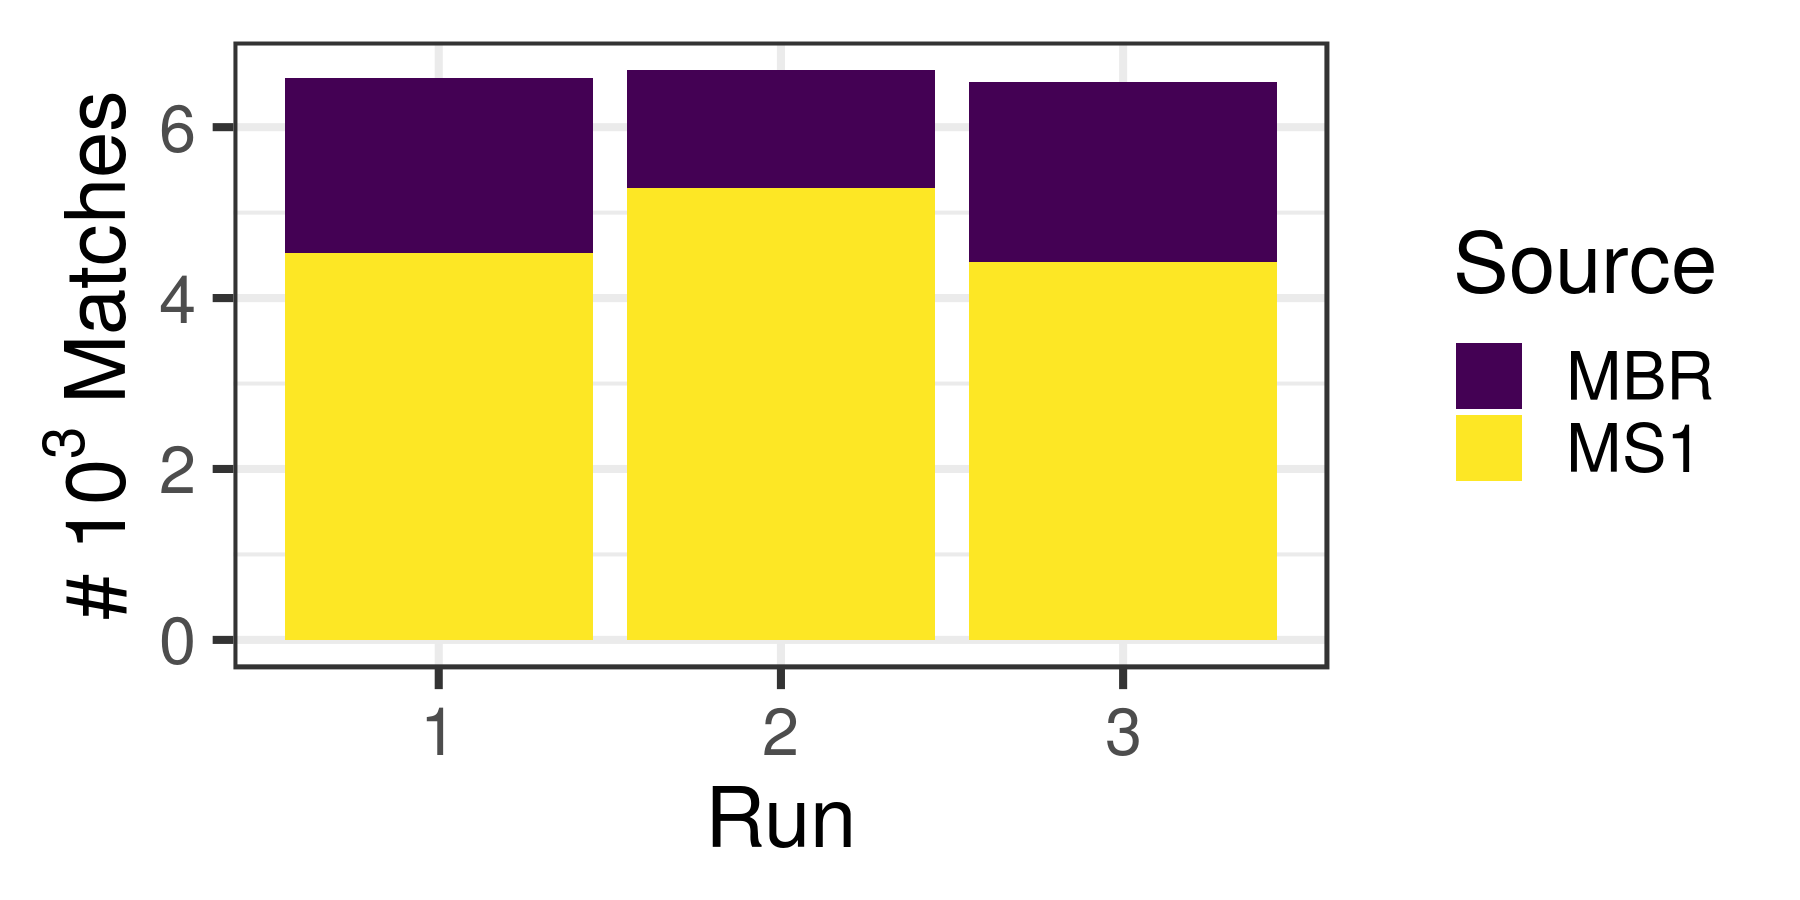
\includegraphics[width=0.5\textwidth]{mbr_summary}
\caption{Count of identifications on each run segreagated by source. More than 4k spectra were identified and validated by SearchGUI+peptideShaker. The MBR acts as an imputation step where extra identifications are performed by gathering the information collected from identifications in other samples and reprocessing the spectra files. As a consequence, more identifications with a lesser fraction of missing datapoints are achieved. In this particular case, hundreds of identifications were accomplished}

\label{fig:mbr_summary}
\end{figure}

\begin{figure}[!h]
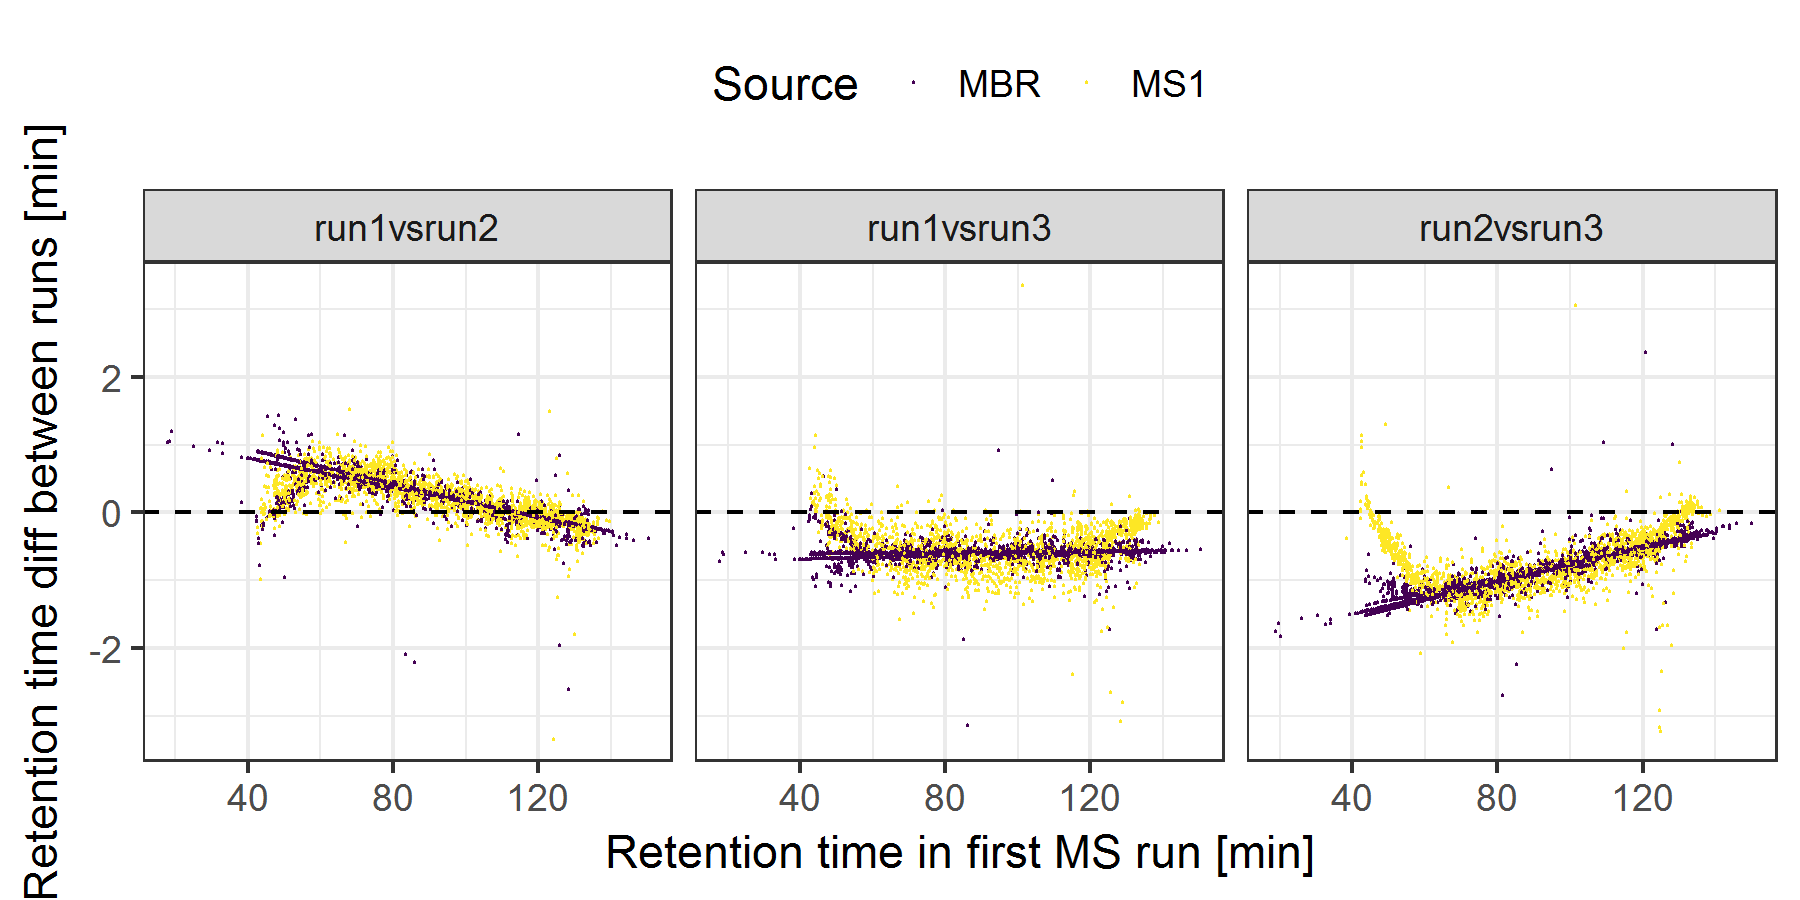
\includegraphics[width=\textwidth]{mbr}
\caption{Match Between Runs with moFF. Every dot represents a peptide shared across 2 runs. The coordinate system illustrates its retention time on the first run on the x axis and the difference with the second run on the y axis. The color depicts whether the identification was carried out during the PSM process, or thanks to a cross-identification achieved by the MBR module.}
\label{fig:mbr}
\end{figure}

Once as many identifications as possible were gathered, a refinement of the measured MS1 intensity can be implemented to select the apex of every peak cluster, which yields robust intensity measurements for each sample (see figure \ref{fig:apex_intensity}). The extracted apex intensity can be used as a proxy for peptide abundance in the following quantification step.

\begin{figure}[!h]
\begin{subfigure}{.9\textwidth}
  \centering
    \caption*{A}
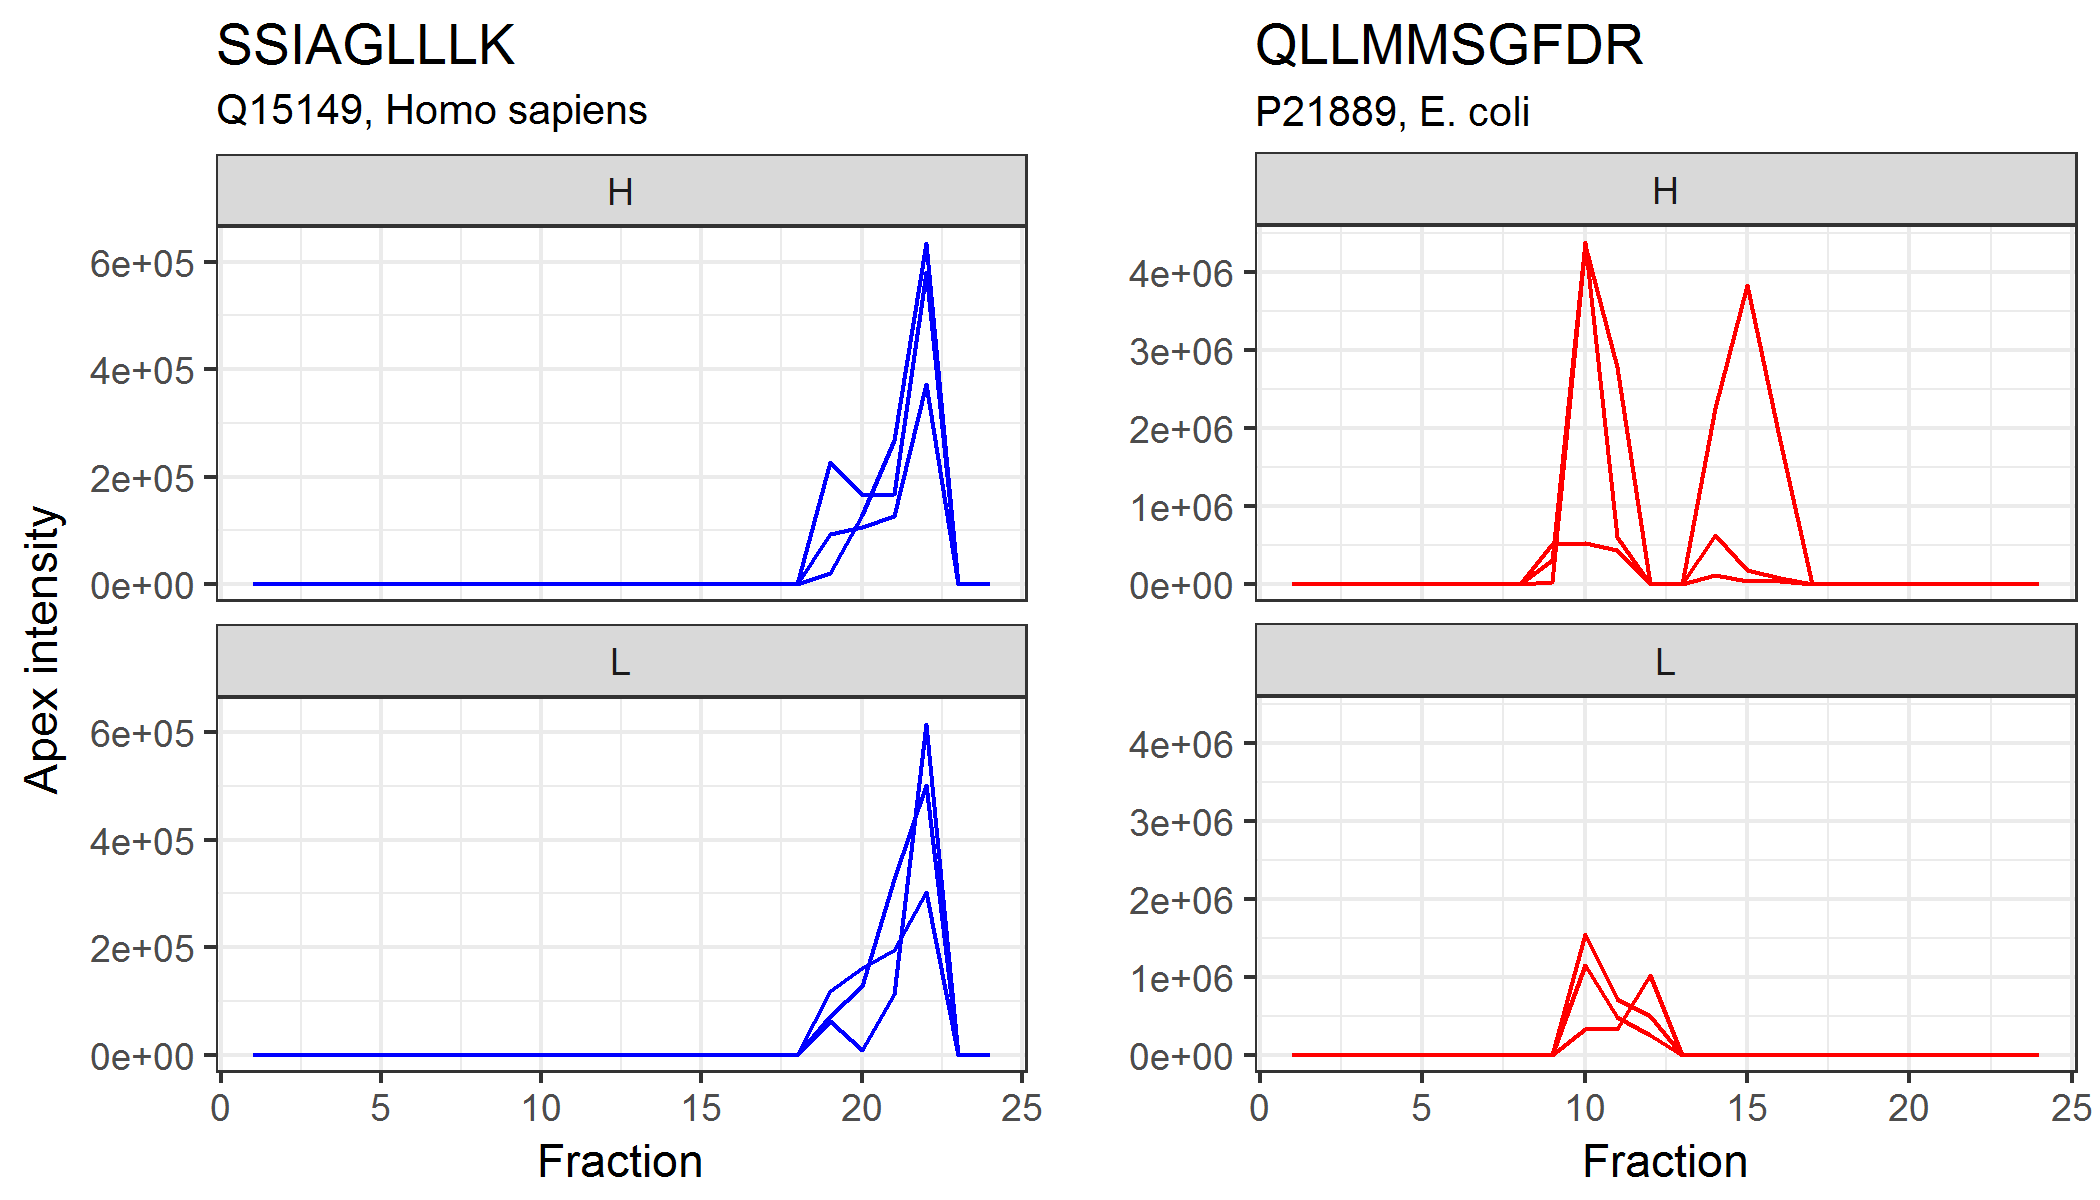
\includegraphics[width=.9\linewidth]{peptide_profile}
\end{subfigure}
\bigskip

\begin{subfigure}{.9\textwidth}
  \centering
    \caption*{B}
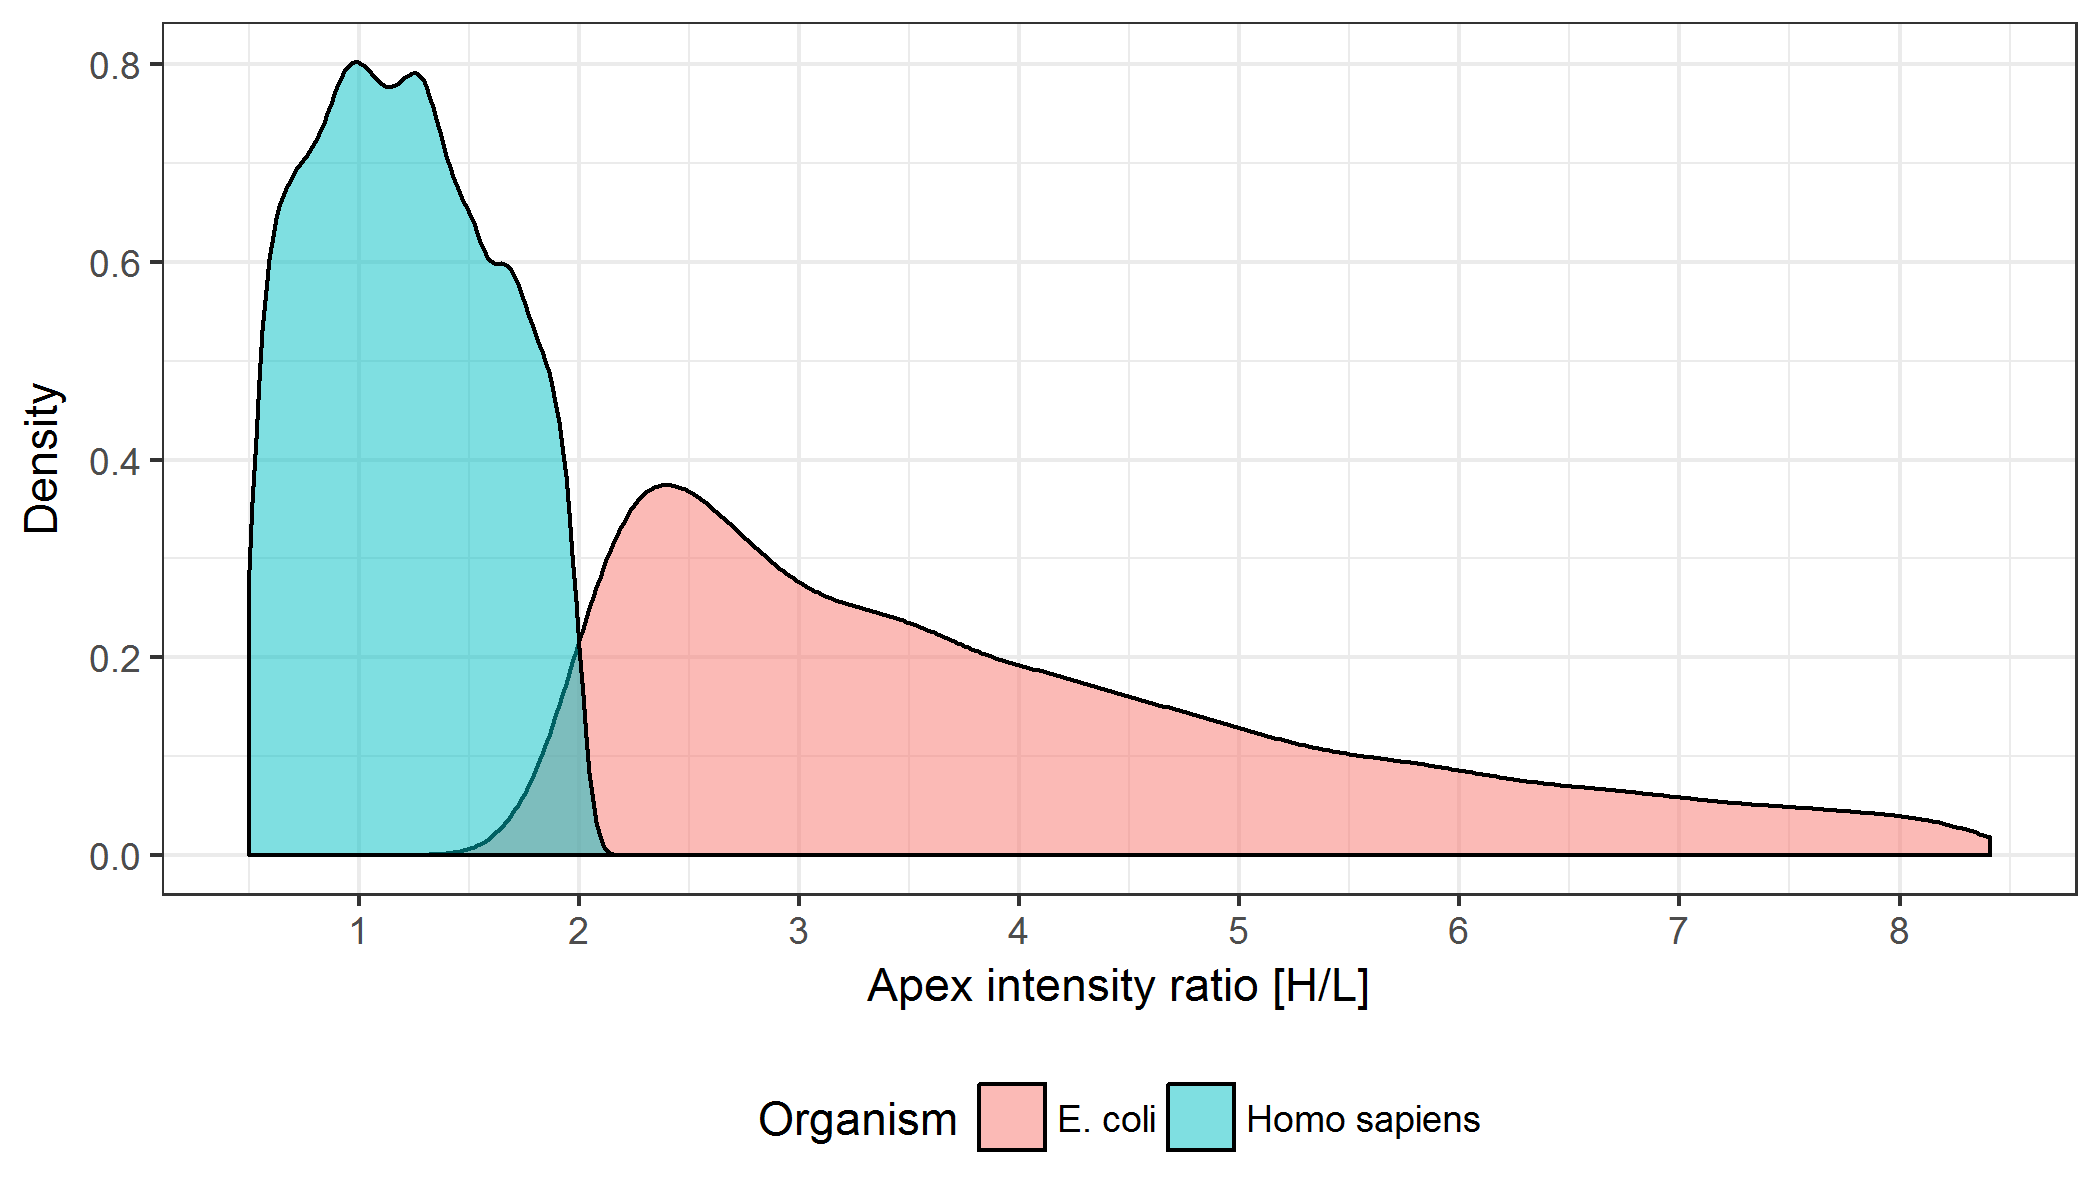
\includegraphics[width=.9\linewidth]{density_ratio}
\end{subfigure}
\caption{\textbf{A} The apex intensity profile across fractions for 2 different peptides, one from \textit{Homo sapiens}, and one from \textit{E. coli}. The figure illustrates the intrinsic intensity variability between technical replicates, particularly in the case of the \textit{E. coli} QLLMMSGFDR peptide, as it was almost non-existent in one of the runs. \textbf{B} The expected pattern of overall similar intensities for the \textit{Homo sapiens} data and 3-fold higher intensities for the \textit{E. coli} data in condition H was observed, confirming the good performance of the protocol.}
\label{fig:apex_intensity}
\end{figure}

\subsection{Quantification}

The result of this step was a table where the $log_2(FC)$ estimate, together with test statistics are returned for every protein group.

\section{Discussion}


\subsection{Improvement of the PSM process}

The low attained matching rate manifests existing room for improvement in the currently available tools CITE THAT. Remarkably, it has been shown that the combined usage of multiple search engines can increase identifications, since the different statistical frameworks implemented in each of them compensate each other\textquotesingle s caveats CITE THAT. Furthermore, \textit{de novo} search engines are available and supported by SearchGUI. Their usage could contribute to further improvements in the identification rate.

The most important reason why many spectra remain unidentified is the presence of post-translational modifications (PTMs), which exponentially increase the search space, forcing most workflows to discard many of the peptides featuring a PTM. New approaches to the problem are emerging, mainly machine learning methods for the handling of unexpected modifications CITE ralf gabriels. Moreover, the prediction of \ac{MS2} peak intensities patterns from peptide sequences promises to increase the amount of evidence available during the PSM process, thus boosting correct identifications CITE MS2PIP.



Finally, the extremely low matching rates in the latter fractions translates to decreased contributions to the number of identifications. This indicated that decreasing the number of fractions would not have had a major impact in the experiment\textquotesingle s depth.


\section{Conclusion}


\chapter{Pipeline benchmarking on \ac{NZ} data}
\label{chap:benchmark}

\section*{Summary}

A benchmark dataset generated by \ac{NZ} technicians was run through the pipeline presented in chapter \ref{chap:pipeline} to showcase its performance. The experiment consisted of the application of two different treatments to THP-1 cell cultures. One group was subjected to an experimental procedure triggering the immunological response, while the other group was subjected to a negative control. The analysis of the resulting dataset through the aforementioned pipeline should thus reflect a change in the protein profile corresponding to an activation of the immune system in the first group when compared to the second. The results confirmed that the computational analysis successfully captured this response. It was concluded that the software can be used in future experiments where the expected biological phenomena is not known.



\chapter{Bayesian modelling of fold change estimates}
\label{chap:model}

\section*{Summary}

The current label-free quantification methods, reviewed in section \ref{sec:quantification} all rely on frequentist statistics, which return point estimates of model parameters such as the estimate of the fold change across conditions. However, a Bayesian based approach to this problem is lacking in the literature. As a response to this shortcoming, a statistical model implemented in the probabilistic programming framework Pymc3 was developed and tested on the same benchmark dataset from chapter \ref{chap:pipeline}). The execution of the three steps required when doing Bayesian modelling, mainly (I) model implementation, (II) computation of posterior probabilities and (III) model checking, will be described for this particular problem in the present chapter, together with a discussion on its usability and its strengths.

\begin{figure}[!h]
\centering
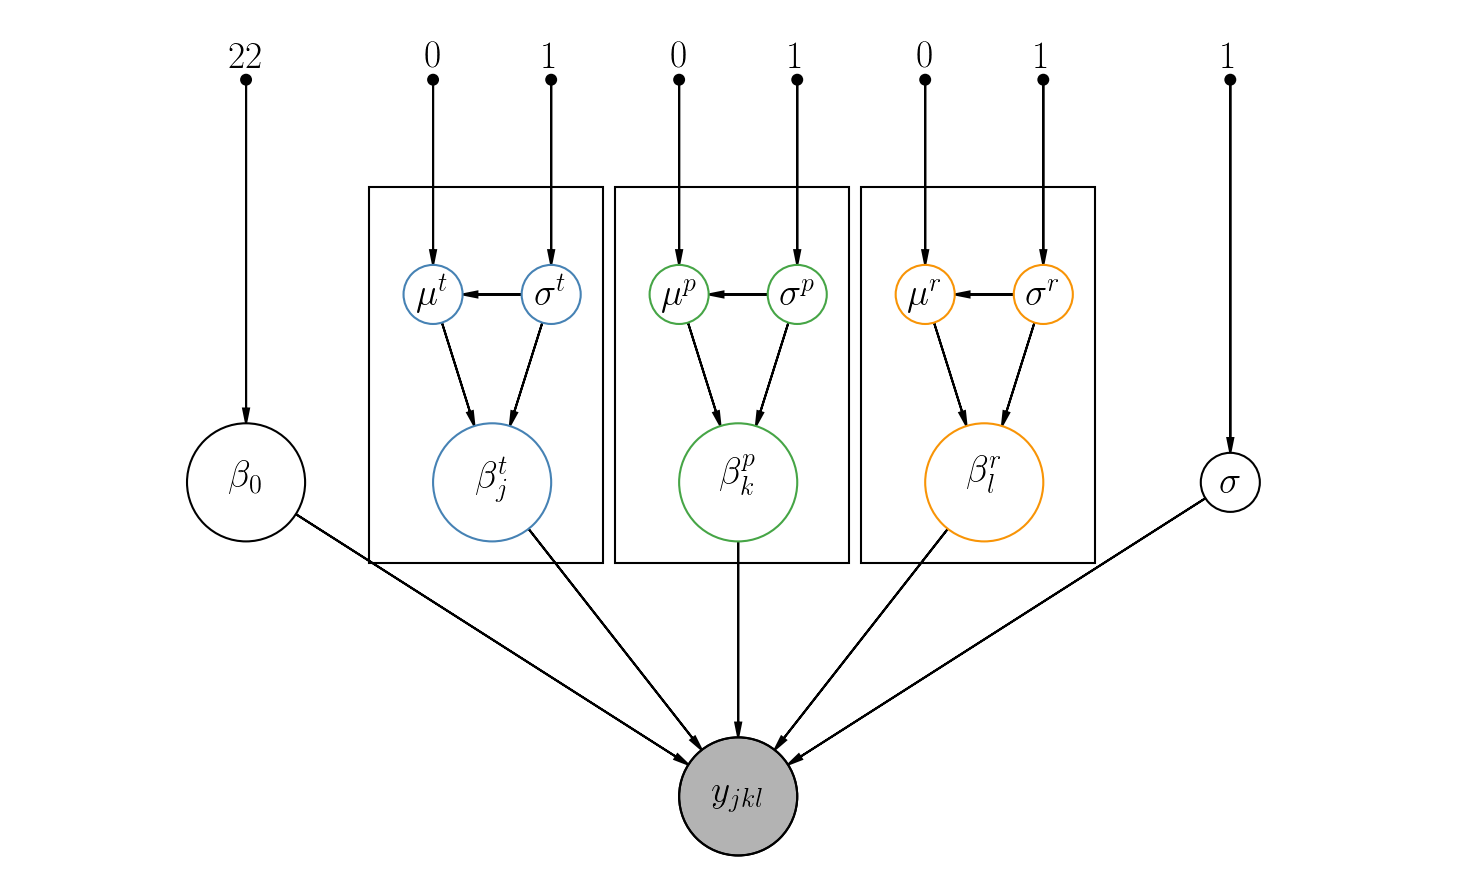
\includegraphics[width=\textwidth]{graph}
\end{figure}

%As such, they are the target of multiple regulatory pathways ensuring their quantities are kept within homeostatic ranges.

\chapter*{Conclusion}
\label{chap:conclusion}

\chapter*{Appendix}
\label{chap:appendix}

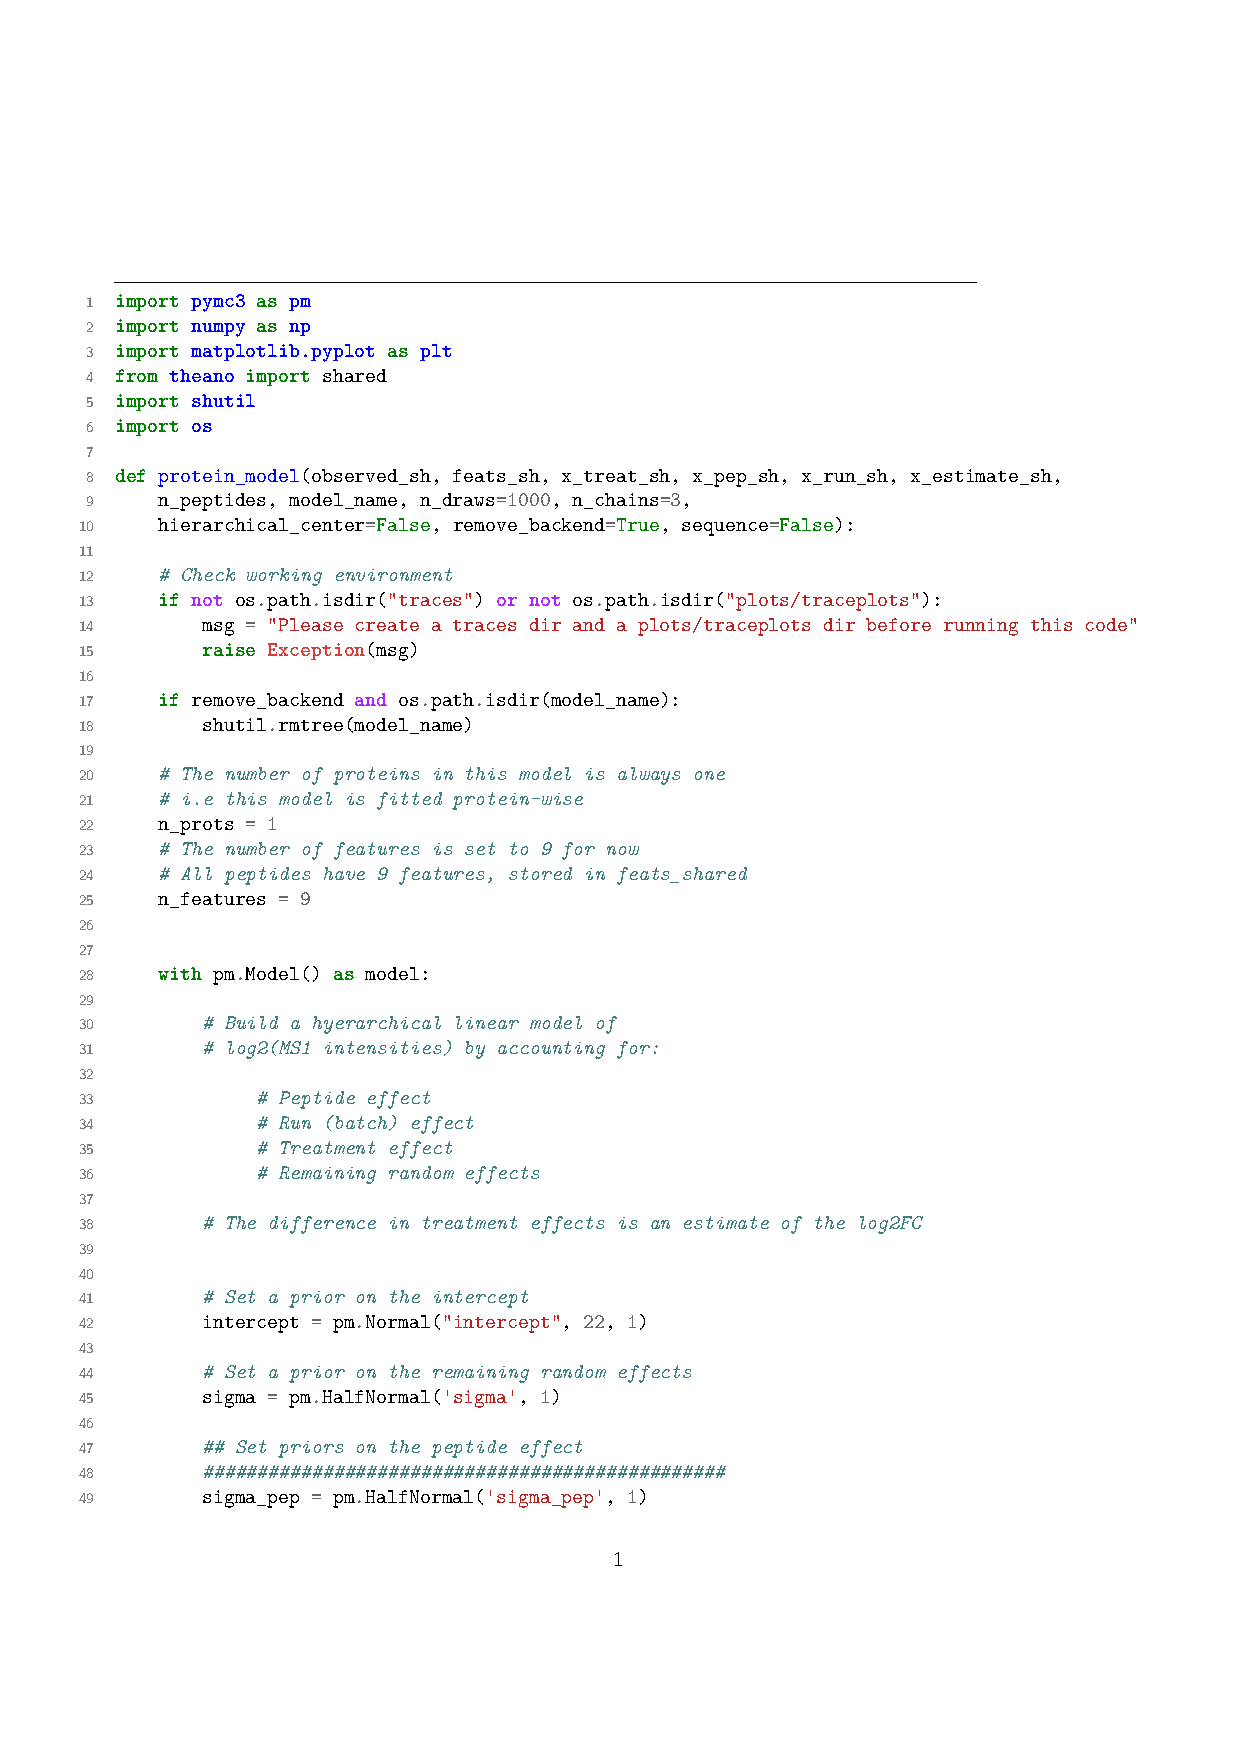
\includepdf[pages=-]{appendix.pdf}


\bibliographystyle{unsrt_etal}
\footnotesize{\bibliography{bibliography}}

\end{document}
%%  ==================================================================
%%  End document

